\section{\systemname Sleep Monitoring Platform}\label{Sec:3design}

%\subsection{Overview of \systemname}

%\begin{figure}
%  \centering
  % Requires \usepackage{graphicx}
 % 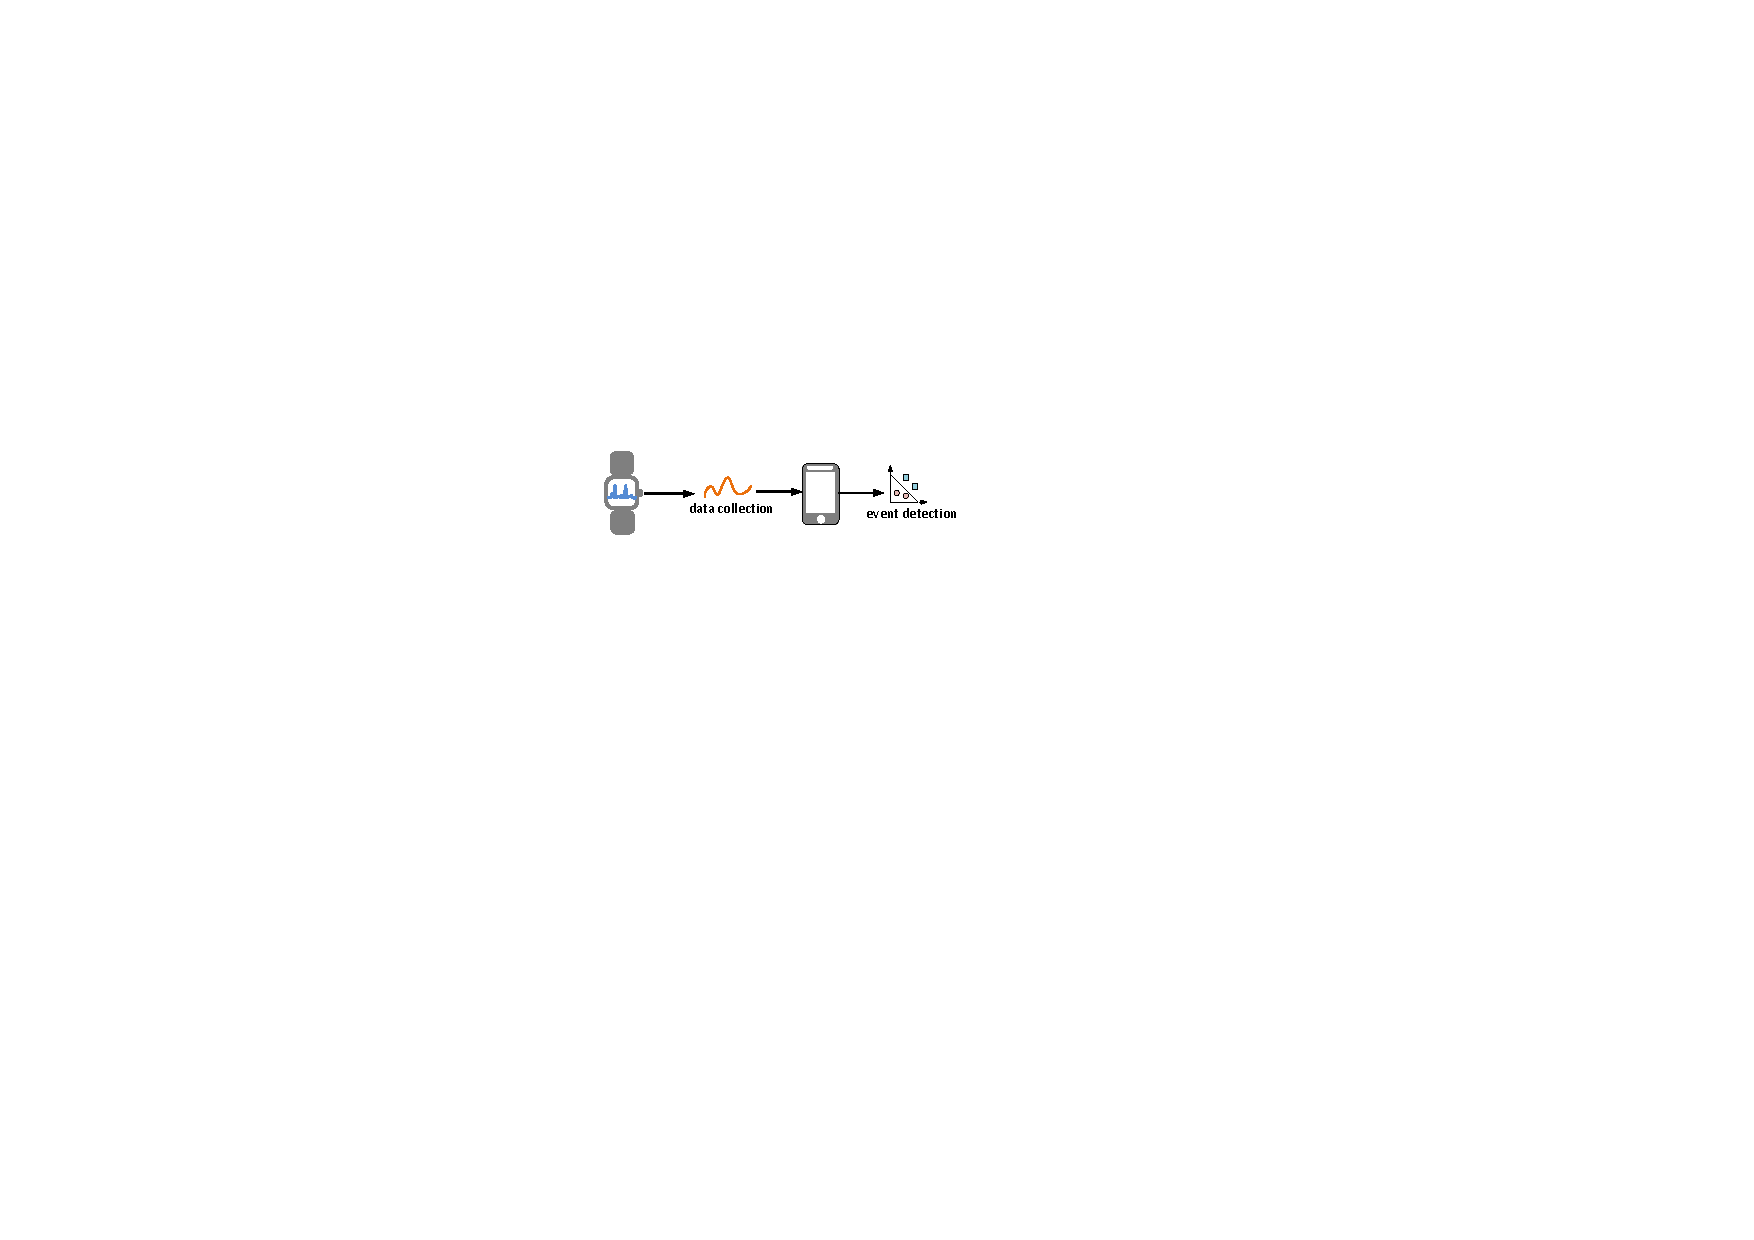
\includegraphics[width=0.7\textwidth]{figures/overviewd.pdf}\\
 %\caption{Overview of our 2-stage approach. Sleep data are collected through smartwatch sensors, which are then passed to be processedby a mobile app
%  to detect sleep events.}\label{fig:overview}
%\end{figure}

\systemname is a novel smartwatch-based sleep monitoring system that aims at estimating sleep quality and capturing rich information about
behaviours and events occurring during sleep. By capturing this information, \systemname can analyze potential reasons for sleep problems
and provide the user with suggestions on how to improve their sleep routine or sleep environment. To achieve its design goal, \systemname
exploits a wide range of sensors that are common on commercial off-the-shelf smarwatches: (i) accelerometer, gyroscope, and orientation
sensor are used to collect body and hand movements; (ii) microphone is used to measure level of ambient noise and to capture acoustic
events; and (iii) ambient light sensor is used to monitor illumination within the sleep environment. The different sensors and information
extracted from them are summarized in Table~\ref{tab:test}. In the following we discuss the different subcomponents of \systemname in
detail.

%acoustic data, the ambient light sensor for illumination conditions, the orientation sensor for calibration. The collected data are
%transmitted to a smartphone via Bluetooth. We propose a set of new analysis and algorithms to effectively detect sleep events from the
%collected data. Table~\ref{tab:test} lists the set of sleep events supported by \systemname.
%Figure~\ref{fig:overview} depicts our 2-stage approach that involves collecting data using a smartwatch and sleep event detection using a
%smartphone. Sleep data are collected using smartwatches sensors. Our work

\begin{table}[t!]
 \caption{\label{tab:test}Sleep events targeted in this work}
 \centering
 \begin{tabular}{ll}
  %\toprule
  \toprule
  \textbf{Event}& \textbf{Type} \\
  \midrule
\rowcolor{Gray}  Sleep postures & Supine, Left lateral, Left lateral, Prone\\
 Hand positions & Head, Chest, Abdomen\\
\rowcolor{Gray} Body rollover & Count\\
 Micro body movements& Hand moving, Arm raising, Body trembling \\
\rowcolor{Gray} Acoustic events & Snore, Cough, Somniloquy  \\
 Illumination condition & Strong, Weak  \\
  \bottomrule
 %\hline
 \end{tabular}
\end{table}

%\begin{figure}[!thbp]
%\centering
%%\setlength{\belowcaptionskip}{-9pt}
%      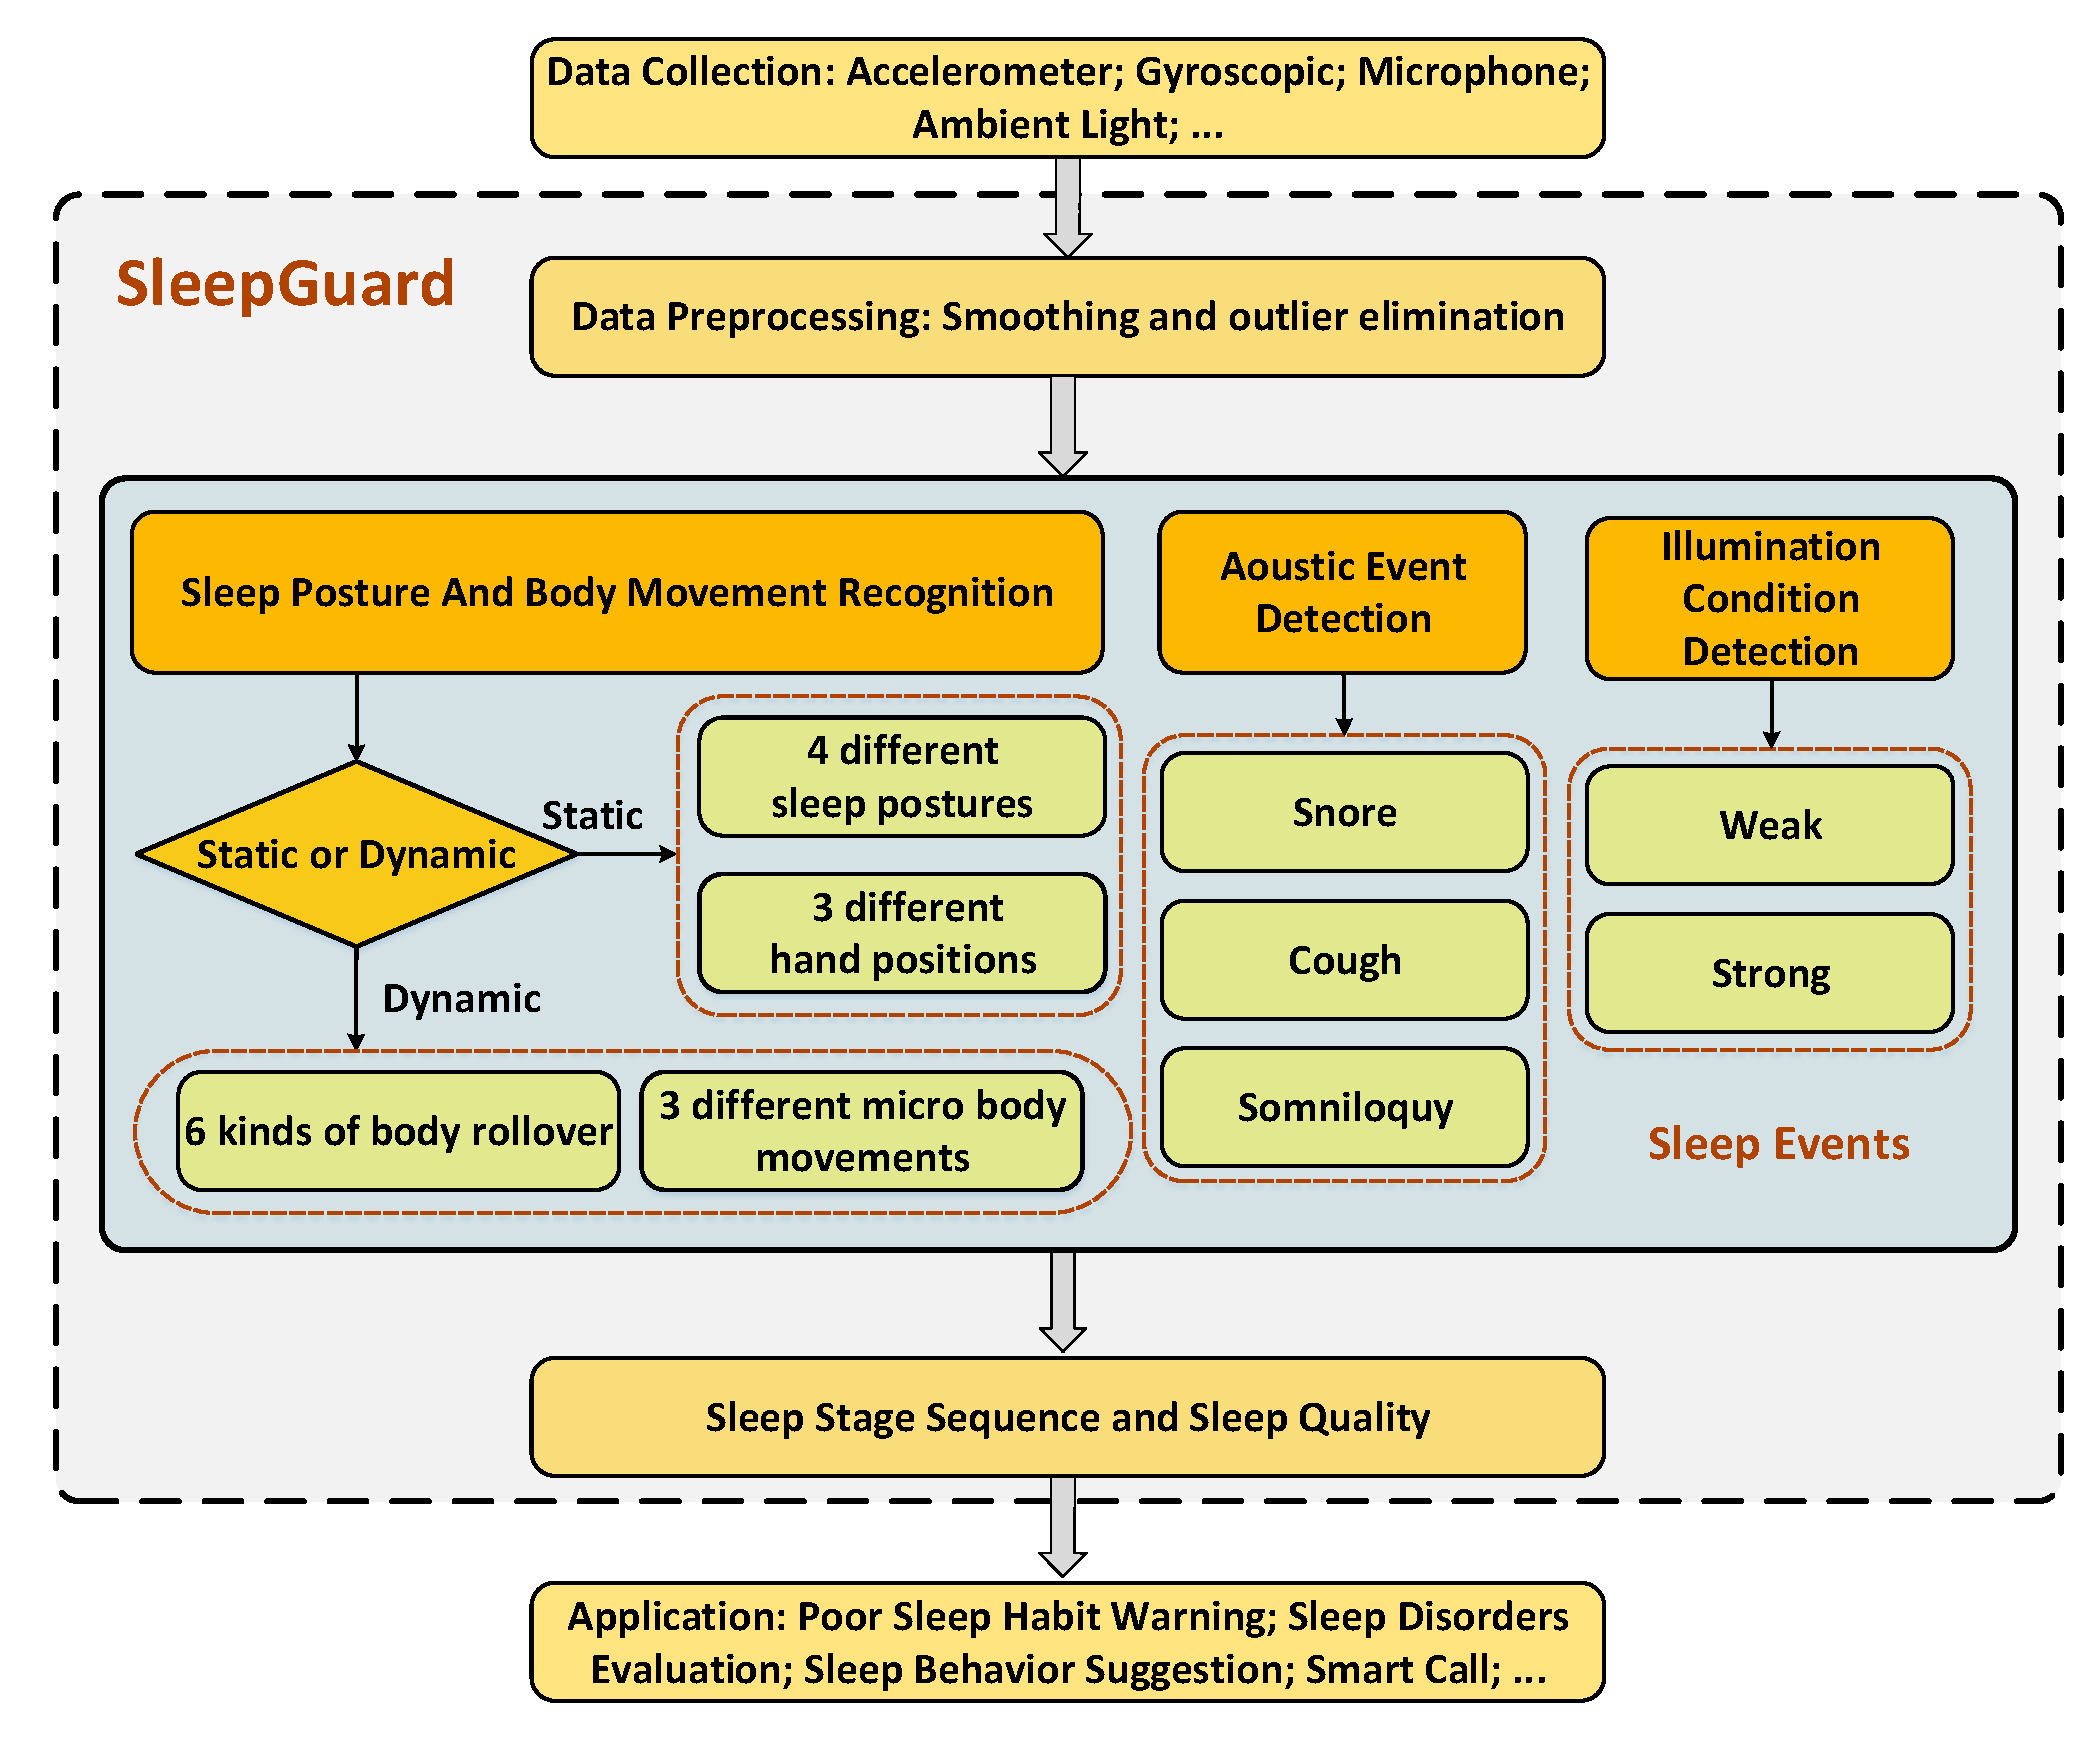
\includegraphics[width=0.97\linewidth]{Figures/SystemFlow.pdf}
%  \caption{System overview of {\systemname}.}\label{fig:overview}
%\end{figure}
%
%
%\begin{itemize}[itemsep=1mm,nolistsep]
%  \item {\textbf{Data Collection and Preprocessing.}} A variety of sensing data are related to sleep events include i) the accelerometer and the gyroscope about the body movement, ii) the microphone measured acoustic sound, iii) the ambient light sensor about the illumination condition, and iv) the orientation sensor with some auxiliary information. The data is collected every 30 ms on the smartwatch and transferred to the server (such as a smartphone) via Bluetooth. We use data smoothing and outlier elimination to reduce noise in the raw sensor readings.
%  \item \textbf{Sleep Event Detection.} A series of novel algorithms are developed to recognize different sleep events. In particular, some key insights are observed about different body postures, body rollovers, hand positions, micro body movements and acoustic events. Note that before identifying those events, {\systemname} first carries out a coarse-grained detection and judges whether the user is lying or not.  After that, we can estimate the user's bedtime. During the user is lying on the bed,  we regard that the user fell asleep if we do not detect a large movement within 20 minutes.
%  \item \textbf{{Sleep Pattern Report.}} Sleep Pattern Report. After we obtain the detected sleep events, we integrate them to the clock information, illumination condition, and then use the Hidden Markov Model to infer the sleep stages and evaluate sleep quality. Different from existing apps on the market, {\systemname} provides detailed procedure about the sleep report. The output of our system, for example, sleep postures and the position of user's hand could be used as input to build a broad range of sleeping quality and  heathy applications, such as poor sleep habit warning, the evaluation of insomnia, nightmare and sleep disorders. With the extensive experiments conducted, we conclude that {\systemname} exhibits a relatively high accuracy comparing to state-of-the-art systems.
%\end{itemize}


%\subsection{Feature Calculation and Selection}
%Appropriate  features  can  reflect  the  potential  information  underlying the  signals. The  features  used  in {\systemname} are shown in  Table \ref{Tab1}. To detect different sleep events, we use two main features. The first one is the movement related features, that are angle of inclination calculated by acceleration data and the angle of rotation calculated by gyroscopic data. Beyond that, to detect different sound events during sleep, we calculate the energy and zero-crossing rate of the sound signal.
%
%\begin{table}[!thbp]
%\centering
% \caption{Calculated Features}\label{Tab1}
%   \renewcommand\arraystretch{1.7}{\multirowsetup}{\centering}
%        \begin{tabular}{c|c|c}
%        \hline
%        {\bf{Data}}  &   {\bf{Feature}} &   {\bf{Formula}}\\
%         \hline
%        {$acc$} & {Tilt Angle}   & $ A_x =\arccos(\frac {acc_x}{acc}) $ \\
%        \hline
%        {$\omega$} &  {Rotation Angle}  & $ \theta = \int\omega $ \\
%        \hline
%        %\multirow{2} {0.1cm}
%        {Sound}  & Energy   &$ E=\sum\nolimits_{n=-\infty}^{\infty}|x^2(n)|$ \\
%         {$x(n)$}  & Zero-crossing  & $Z$ \\
%          \hline
%\end{tabular}
%\end{table}




\begin{figure*}
	\centering
	\begin{minipage}[t]{.33\textwidth}
		\centering
		  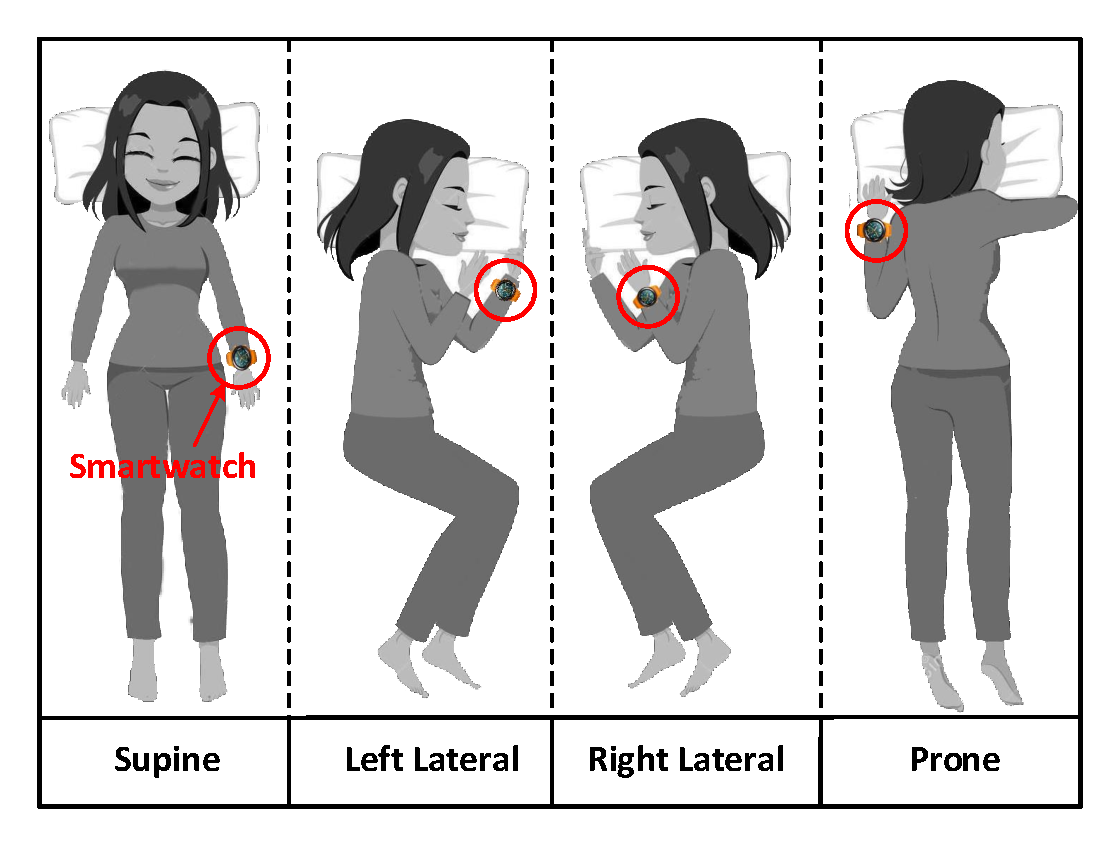
\includegraphics[width=4.7cm,height=3.7cm]{Figures/BodyPosture.pdf}
		\caption{Four sleep body postures.}
		\label{fig:BodyPosture}
	\end{minipage}%
	\begin{minipage}[t]{.33\textwidth}
		\centering
		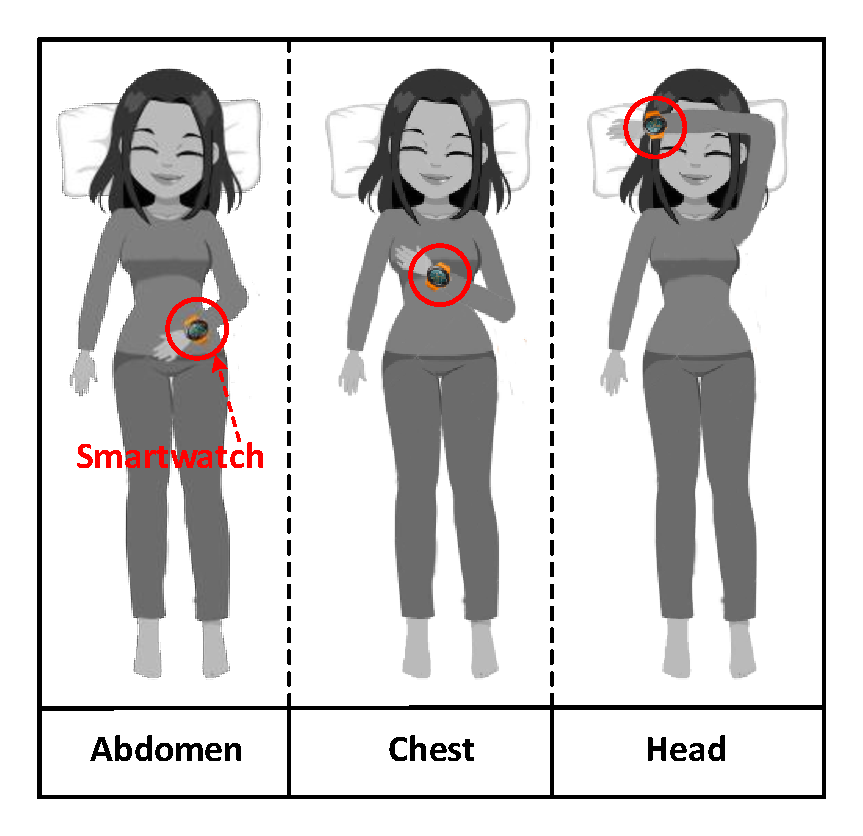
\includegraphics[width=4.1cm,height=3.4cm]{Figures/HandPosition.pdf}
		\caption{Three hand positions.}
		\label{fig:HandPosition}		
	\end{minipage}
\begin{minipage}[t]{.33\textwidth}
		\centering
	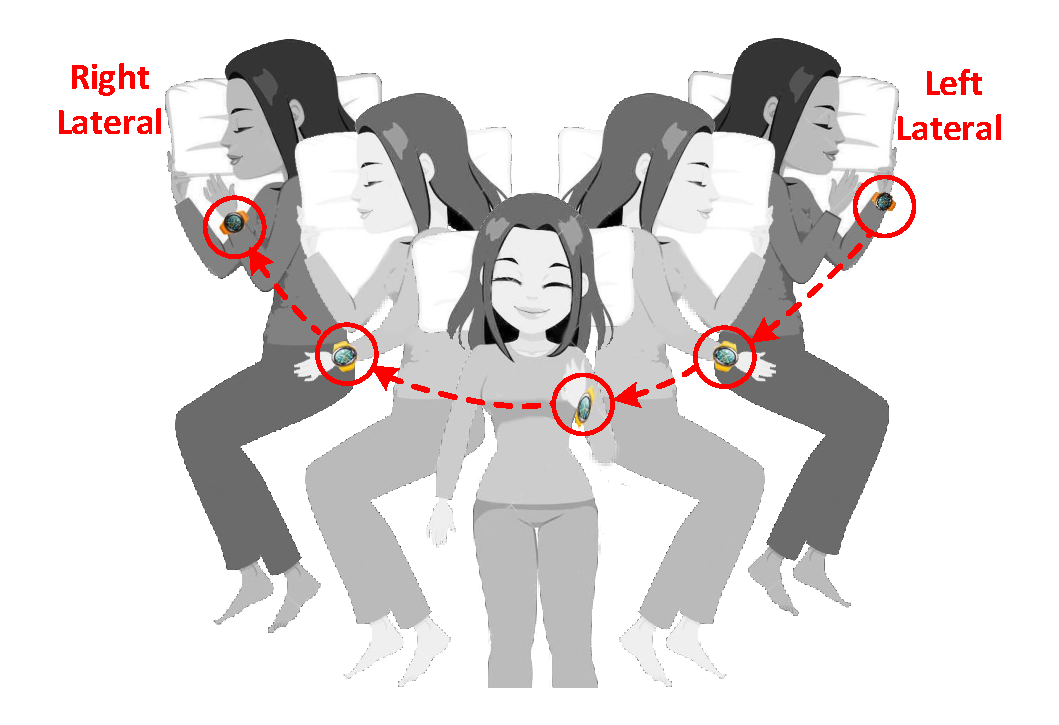
\includegraphics[width=4.7cm,height=3.7cm]{Figures/BodyRollover.pdf}
	\caption{Body rollover from the left side to the right side.}
	\label{fig:BodyRollover}
\end{minipage}
\end{figure*}


\subsection{Training Data\label{sec:trainingdata}}
\textcolor{cyan}{ The training examples used to train our algorithms and to determine the algorithm parameters are collected from 10 users
(5 males and 5 females), aging between 16 and 60. Our testing users were asked to wear a smartwatch to sleep and collected the sensor data
while they were sleeping. Every testing user contributes 10 nocturnal sleep data over a two-week period. We stress that these users are
different from those took part in our evaluation} (Section~\ref{sec:evalusers}).

\subsection{Detecting Sleep Postures and Movements}

One's sleeping position, also referred to as {\em sleep posture}, and the extent of body movements are important factors in determining
overall sleep quality. Suboptimal posture has been shown to affect the severity of sleep disorders and is widely used in medical diagnoses
to analyse effects of sleep disorders~\cite{oksenberg1998effect,eiseman2012impact} while having a good sleep posture has been shown to
correlate with subjective assessments of sleep quality~\cite{dekoninck83sleep}. Similarly, high degree of body movements during sleep
likely reflects restlessness, which results in poor sleep quality. {\systemname} uses motion sensors (accelerometer, gyroscope, and
orientation sensor) to capture user's sleep posture and habits. In the following we detail the techniques we use for capturing the body
posture and movements.  {\systemname}, currently supports the 4 basic sleep postures (see Fig.~\ref{fig:BodyPosture}); 3 hand positions
(see Fig.~\ref{fig:HandPosition}); 6 types of body rollovers (see Fig.~\ref{fig:BodyRollover} for an example); and 3 types of body micro
movements. %These events comprehensively and highly relate to the sleep stages and quality.


\subsubsection{\textcolor{cyan}{Sleep Posture Detection}\label{sec:sleeppdet}}

Dreaming and sleep quality are associated with underlying brain functions, which in turn are affected by body posture~\cite{posture2004}.
Sleep posture also varies across individuals and should fit personal and physical needs of the individual~\cite{posture2016,posture2017}.
For example, sleeping in a prone position is unsuitable for people with ailments, such as heart disease or high blood pressure. On the
other hand, people can consciously avoid postures that would be beneficial for health and sleep quality~\cite{posture2015}. Having an
effective way to detect the current posture and track changes in it would thus be essential for estimating overall sleep quality, and
avoiding potential harm. \systemname captures the four basic sleep postures, which are supine, left lateral, right lateral, and prone. This
is illustrated in Fig.~\ref{fig:BodyPosture}. However, detecting these postures using a single wrist sensor is non-trivial because the
sensor cannot accurately track the entire body movement. We observe that the arm position strongly correlates to the sleep postures, i.e.,
the arm is typically located in a specific, stable location for a given sleep posture. This observation suggests that we can first identify
the user's arm position and the duration of a specific arm location, and then map the information to a sleep posture. Later in this paper,
we show that our approach can achieve a high accuracy in identifying sleep postures.




%\textcolor{blue}{As we all know, it is very difficult to use only a smartwatch to describe
%the posture of the entire body, but we found a key basis for sleeping posture detection through observation and a pilot (see Sec. 3.1).}
%The key intuition for distinguishing between these postures is that arms have common and (reasonably) stable positions in each posture.
%\textcolor{blue}{Thus, we can build a mapping between the user's arms position and sleeping postures and identify the user's posture by
%identifying periods where the hand is in a position that correlates with a specific posture.} The basic idea is similar to the posture
%recognition used in~\cite{sleepmonitor}, but we use an additional step to improve the accuracy of distinguishing between supine and prone
%positions.

To separate sleep postures, {\systemname} considers a set of feasible hand positions for each posture. In the supine position, we assume the user's hand to be on the left side of the body, on the abdomen, on the chest or on the head; in the left and right lateral positions, we assume the user's hand is close to the pillow, on the chest or on the waist. Finally, in the prone position we assume the user's hand is on the side of the head or above his/her head. These positions were selected based on a pilot carried out in our test environment (see Sec.~\ref{sec:expsetup}). Fig.~\ref{fig:BodyPosture} shows one possible hand position for each of the postures.

\begin{figure}
	\centering
	\subfigure[Supine]{
		\label{fig:Supine}
		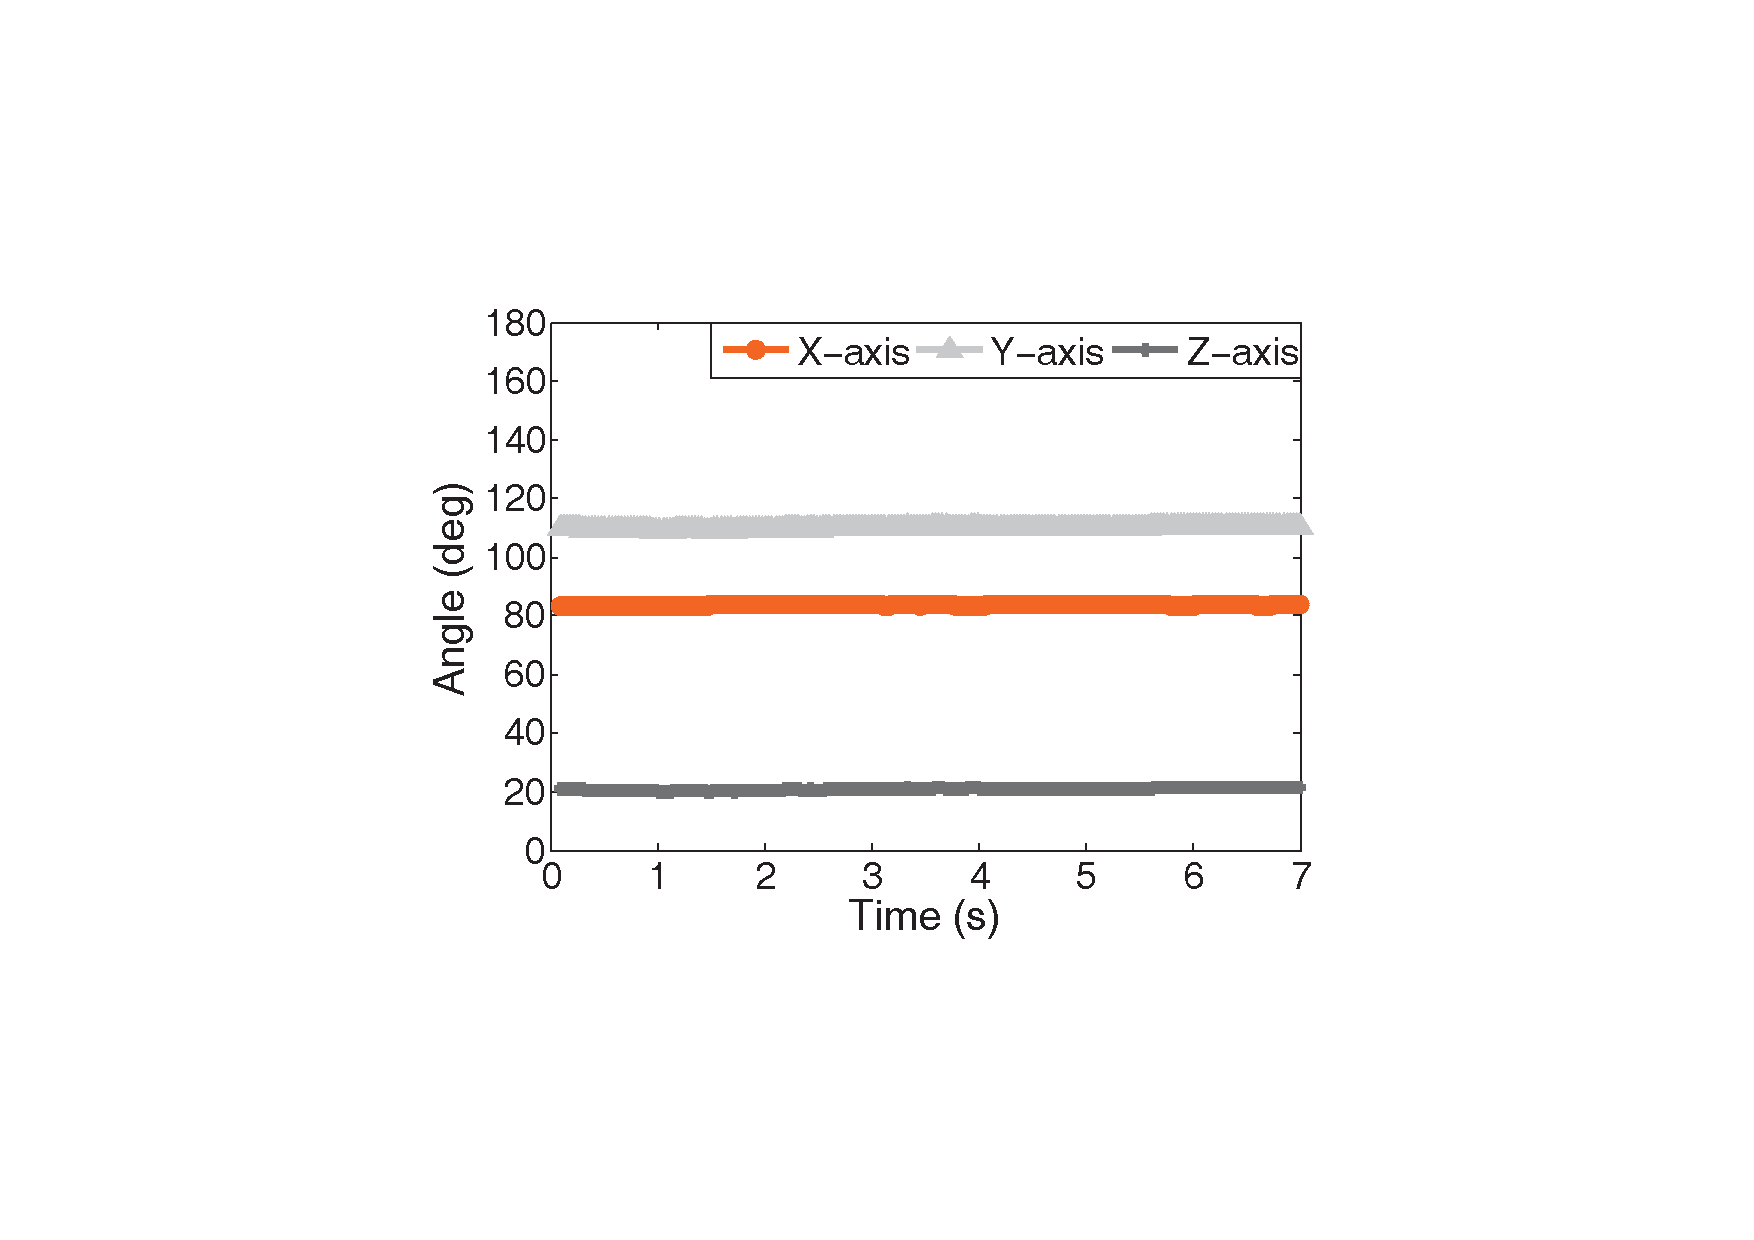
\includegraphics[width=0.24\linewidth]{Figures/Supine.pdf}}
	\hfill
	\subfigure[Left Lateral]{
		\label{fig:LeftLateral}
		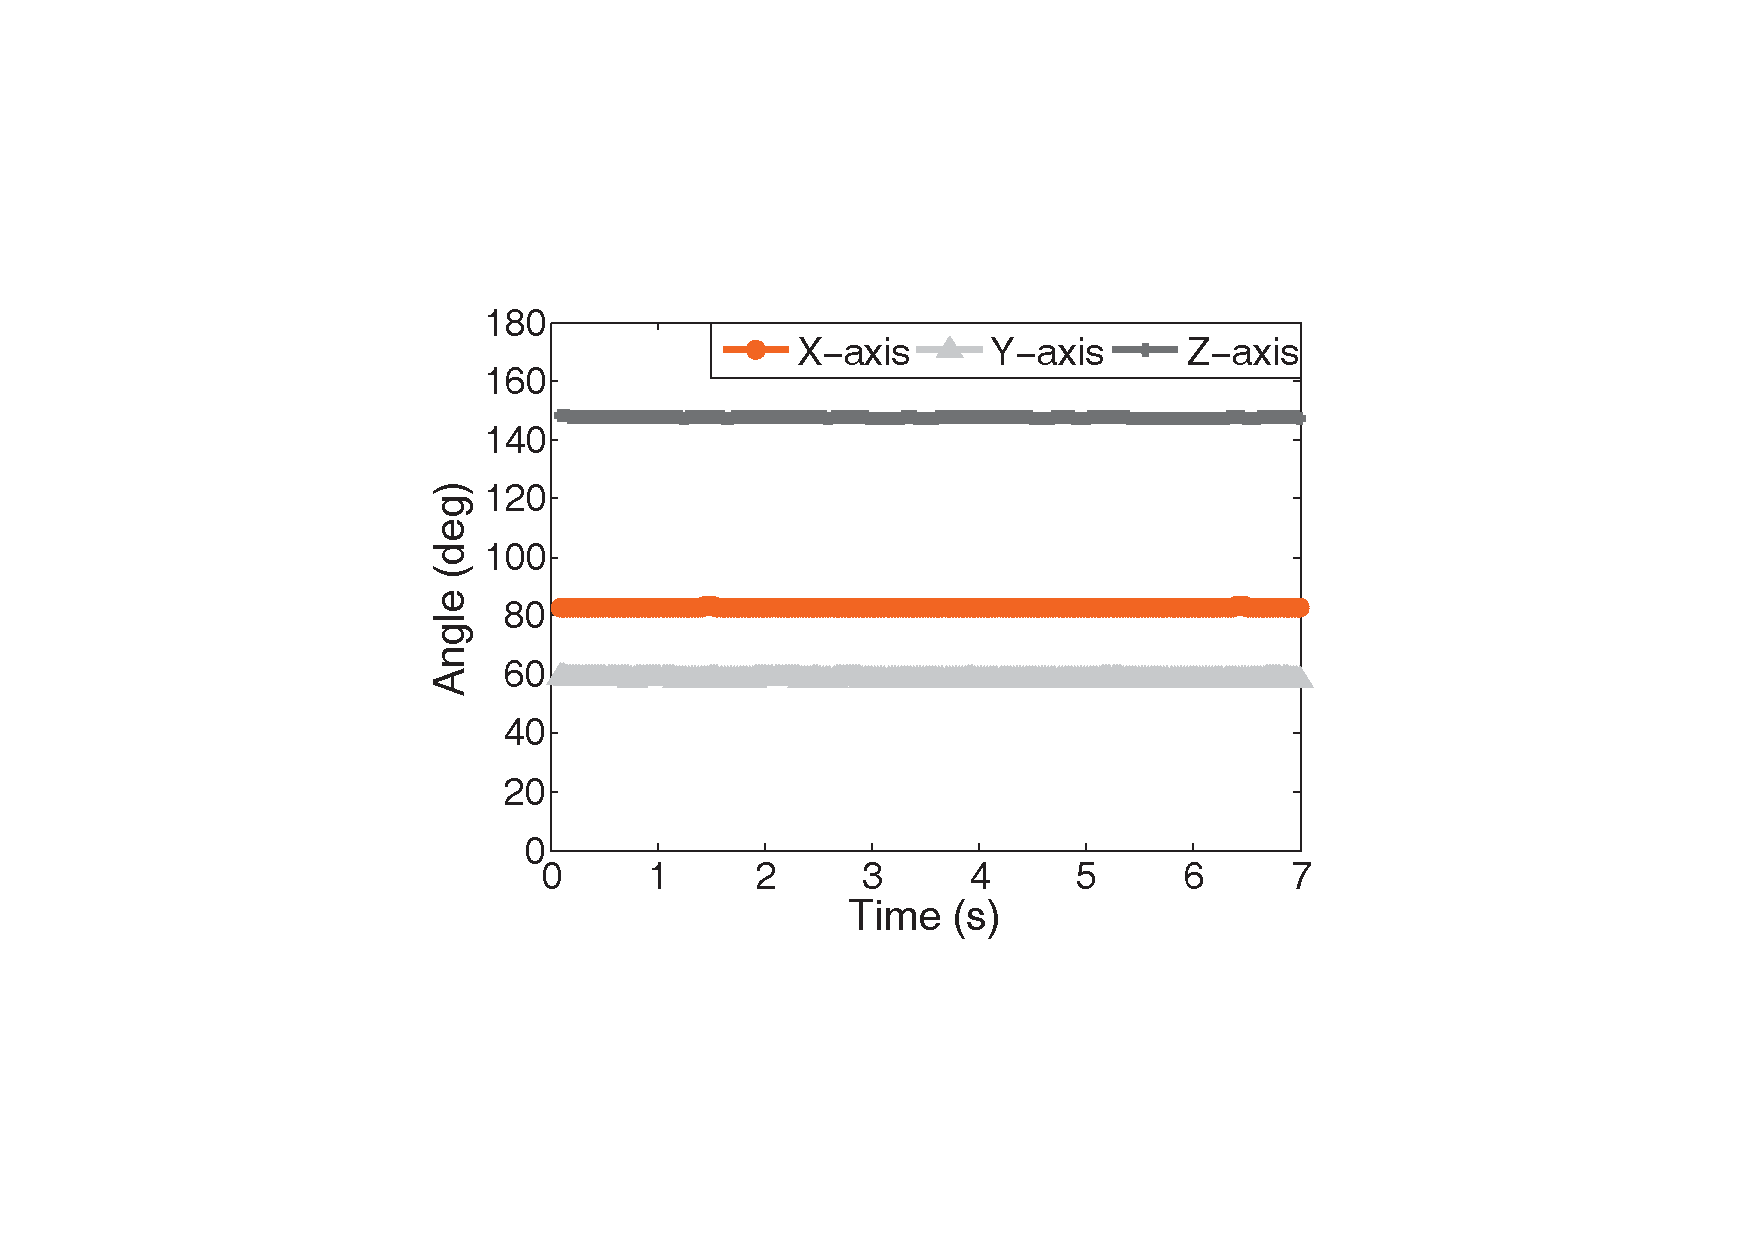
\includegraphics[width=0.24\linewidth]{Figures/LeftLateral.pdf}}
	\subfigure[Right Lateral]{
		\label{fig:RightLateral}
		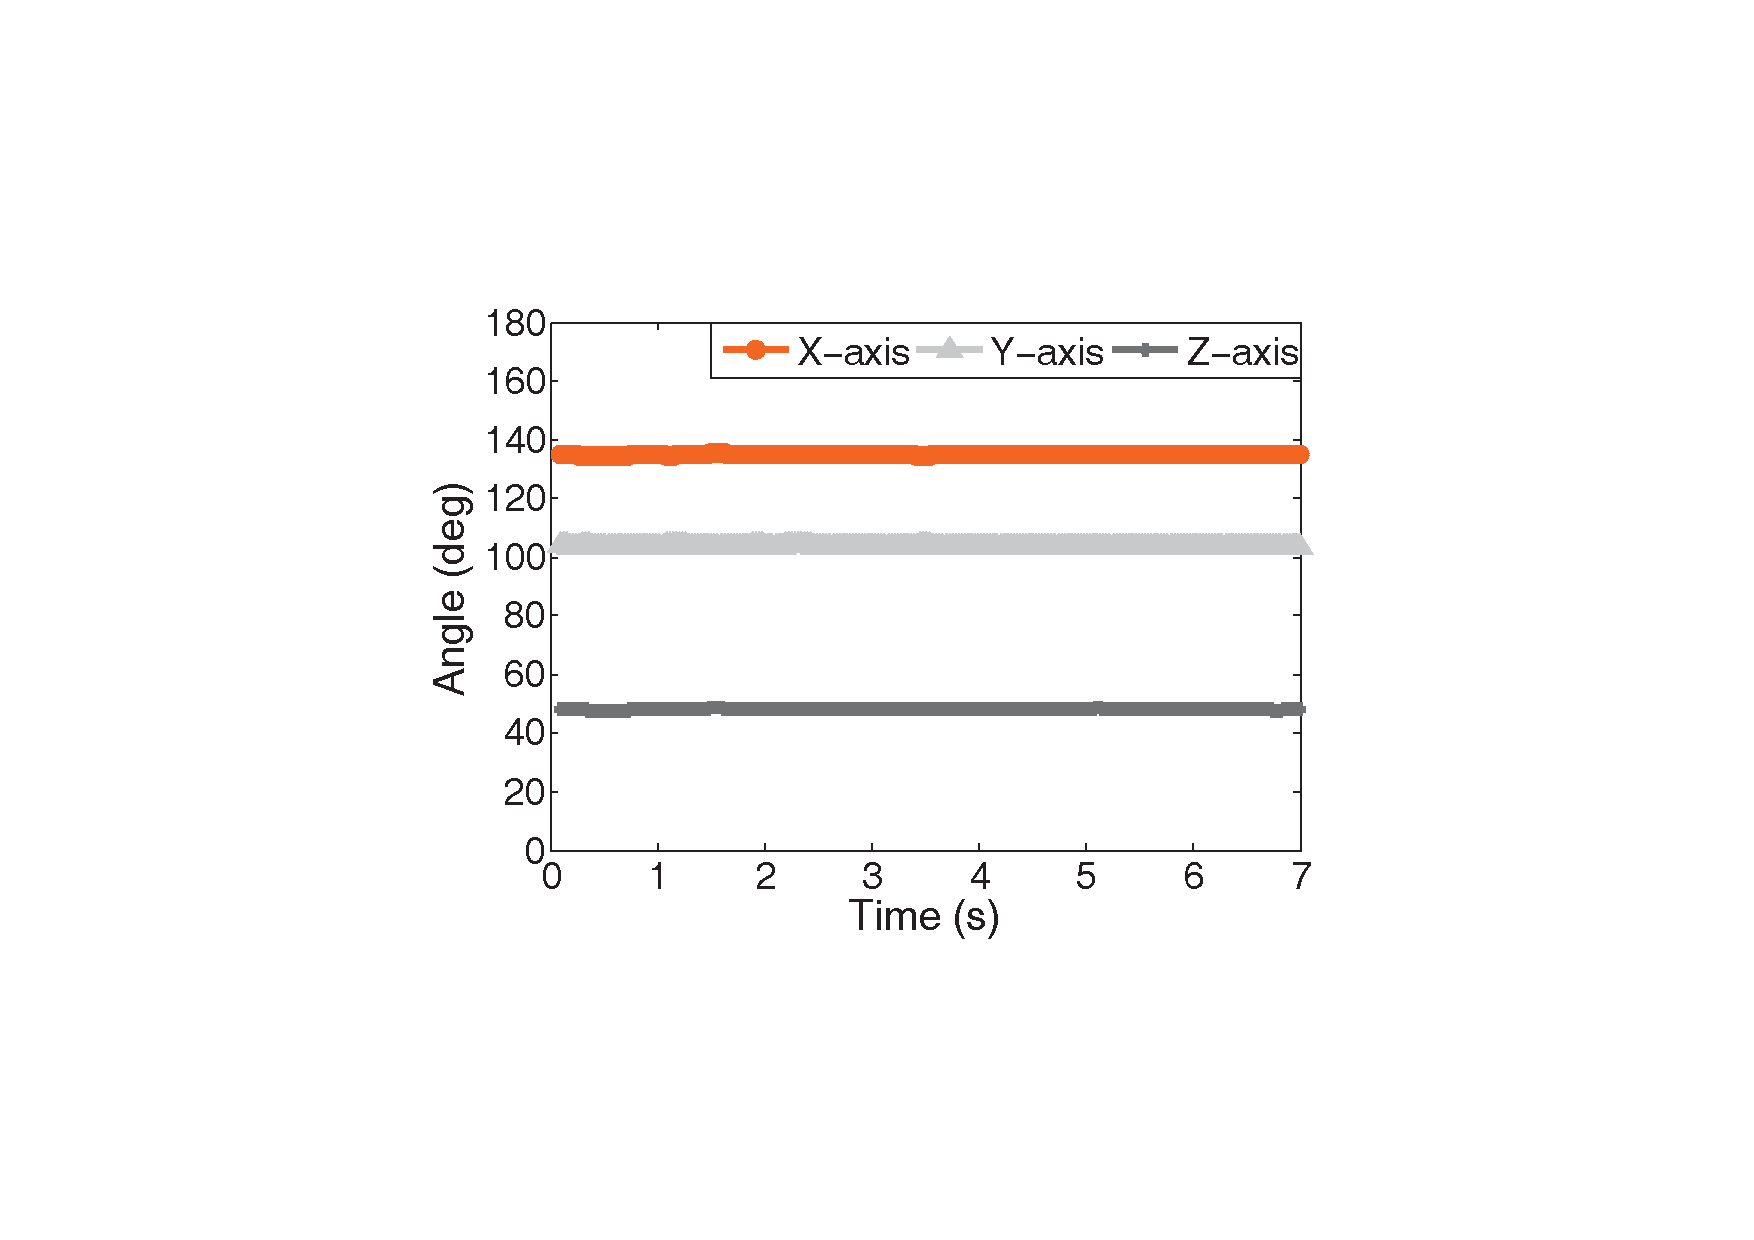
\includegraphics[width=0.24\linewidth]{Figures/RightLateral.pdf}}
	%\hspace{1in}
	\hfill
	\subfigure[Prone]{
		\label{fig:Prone}
		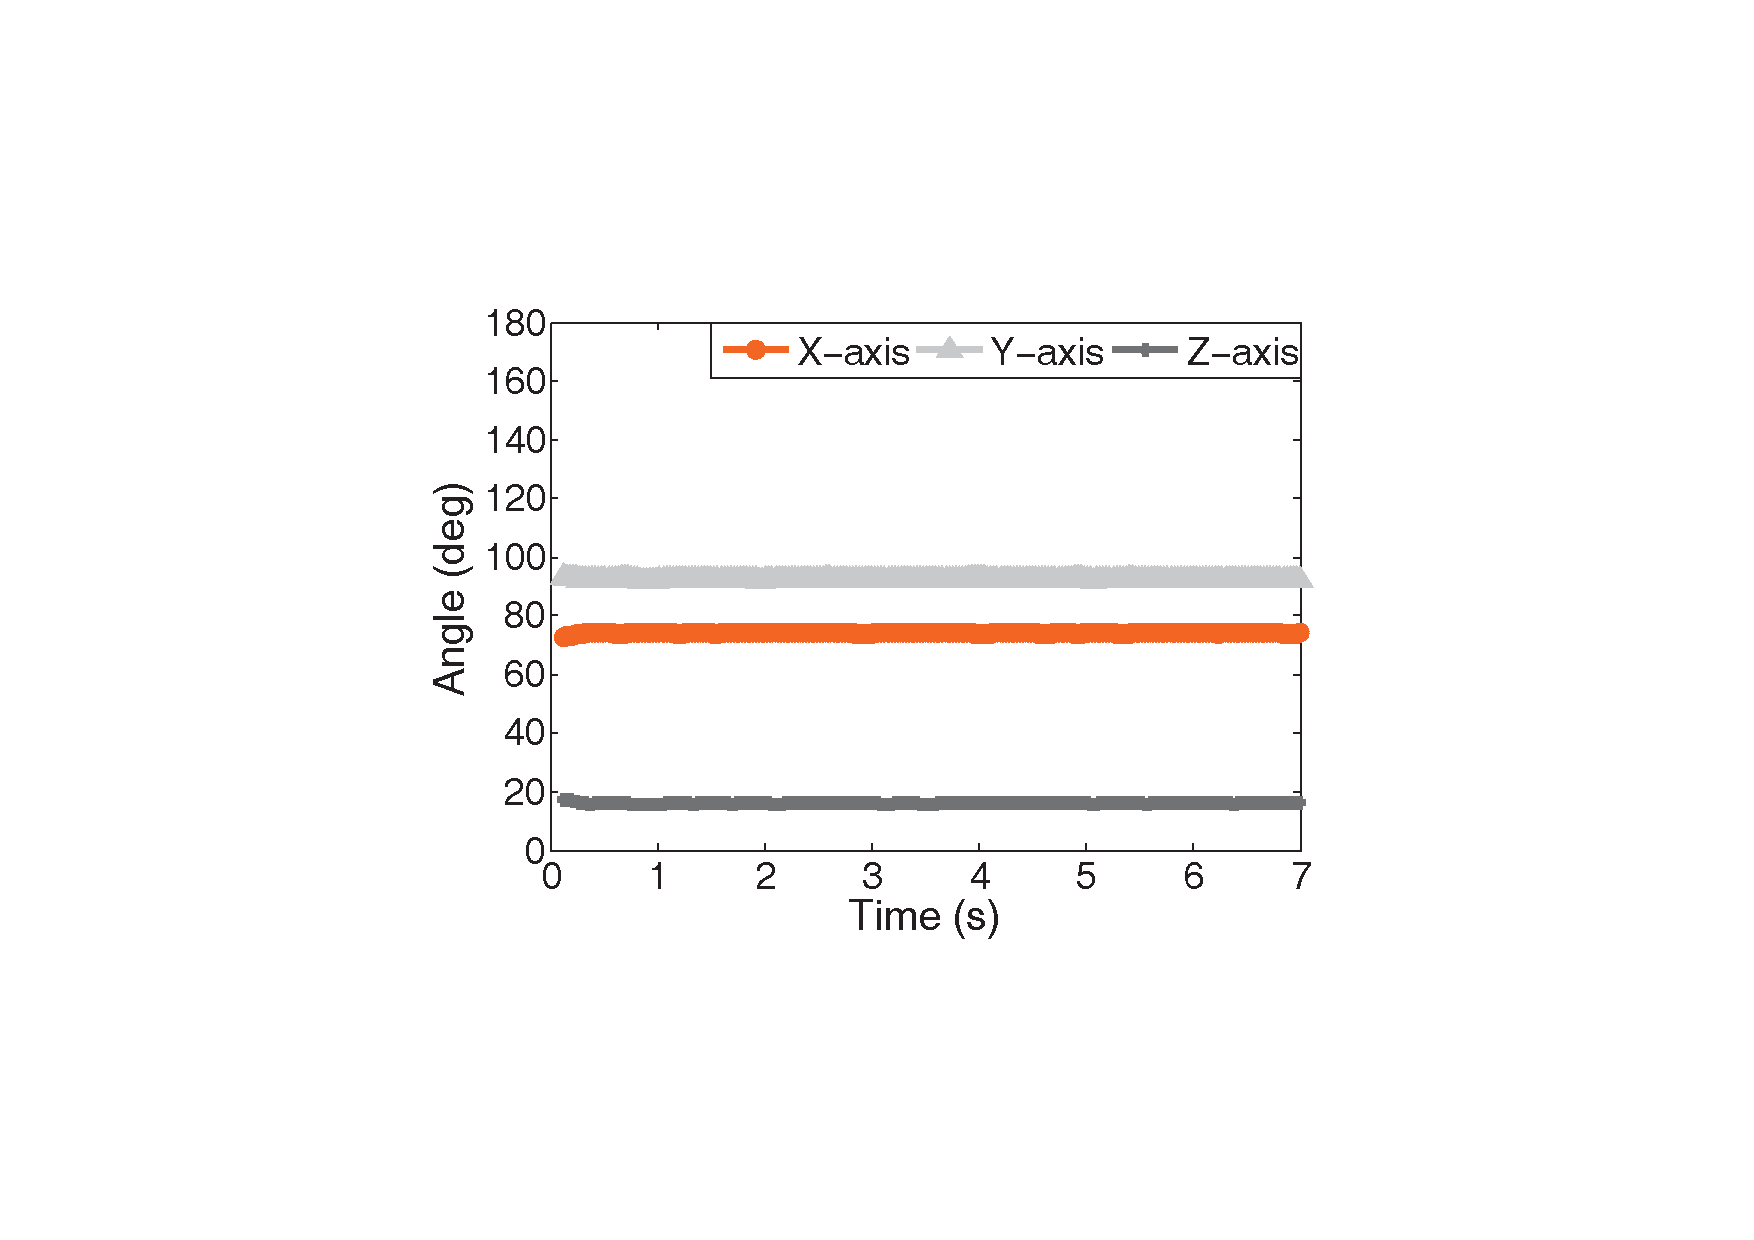
\includegraphics[width=0.24\linewidth]{Figures/Prone.pdf}}
	\caption{The tilt angle characteristics of four body postures.}
	\label{fig:posture}
\end{figure}

%e use a supervised classifier to  And then we use a supervised learning method to create a sleep posture profile. Specifically, we collect training data to create a mapping (i.e., angle mapping) between the angles and the arm under different positions.

Similarly to SleepMonitor~\cite{sleepmonitor}, we use tilt angles readings from three dimensions to detecte postures. We use a K-nearest
neighbour (KNN) classifier, where $k$ is set to 1,  to determine which of the targeting postures that a input feature vector corresponds
to. To determine which posture an input feature corresponds to, we find which of the four posture profiles (i.e., a tilt angle value) is
closest to the input data. The posture profiles used for this task are collected from our pilot study involved 10 users who are different
from the ones took part in our evaluation. To identify which of the postures the data collected within a time window corresponds to, we
average all the calculate tilt angle values of that window. To determine which posture an input feature corresponds to, we find which of
the four posture profiles (i.e., tilt angle values in three dimensions) is closest to the input data. The posture profiles used for this
task are collected from our pilot study involved 10 users who are different from the ones took part in our evaluation. To identify which of
the postures the data collected within a time window corresponds to, we average all the calculate tilt angle values of that window in each
dimension. We then calculate the Euclidean distance of the input values to each of the profiles across the three dimensional to find which
profile is closest to the input values. We then use the body posture associated with the nearest neighbor as the detection outcome.




Fig. \ref{fig:posture} shows the angle values of the four sleep postures targeted in this work. This diagram suggests that the tilt angles
of three axes have obvious differences. The sleep posture thus can be inferred based on the position of the smartwatch and the created
angle mapping. However, a limitation of this approach is that the hand positions during supine and prone postures are similar when the hand
is located on the side of the head (Fig. \ref{fig:Supine} and \ref{fig:Prone}), thus the classification accuracy will be affected.

To improve detection accuracy between supine posture and prone postures, \systemname integrates orientation data as auxiliary feature. This is based on the observation that hand directions in the supine and prone positions are different. When the result of the previous step is prone or supine, and the hand is detected to be located next to the body, we combine the tilt angle with three axes data obtained from the direction sensor as a new feature, and classify these postures using a template-based distance matching approach. Specifically, we return the position corresponding to the template with minimum Euclidean distance with current sensor measurements as the user's posture. %Note that when we use the direction sensor, we must limit the pillow orientation remaining unchanged (in the experiment our pillow is placed on the north). In fact, this assumption can be easily satisfied since most people usually have fixed sleep directions.


\subsubsection{Hand Position Recognition\label{sec:handpr}}

The hand position during sleep can disclose potential health problems, and an improper hand position can even result in health issues~
\cite{position2014}. For instance, placing the hand on the abdomen may indicate discomfort whereas placing the hand on the chest can
increase the likelihood of nightmares due to long-term pressure on the heart. Similarly, placing the hand on the head can put excess
pressure on shoulder nerves and cause arm pain as blood flow is restricted. This can lead to eventual nerve damage, with symptoms including
a tingling sensation and numbness \cite{position2014}.


{\systemname} is designed to recognize three common hand positions -- if the hand is placed on the abdomen, chest or head when the user is
in the supine posture, as shown in Fig. \ref{fig:HandPosition}. We have chosen these three hand positions because there are found to be the
most common and representative positions in our pilot study (Section~\ref{sec:implementation}). Our hand position recognition algorithm is
based on sensor data of rotation angles, tilt angles, and respiratory events. It works by first using the rotation and tile angles to
detect if the hand was placed on the head. If the hand was detected to be not put on the head, it then uses the respiratory events to
detect if the hand was placed on the abdomen or the chest, but not elsewhere before it utilizes the rotation angles to distinguish the
abdomen position from the chest position. We now describe how to detect each of the three positions in more details.




%\textcolor{blue}{The reason why we choose these three hand positions is that they are found to be the most common and representative
%positions during our pilot study (see Sec. 3.1), and they are really related to sleep and health.} Note that as the hand is mostly on the
%bed in prone and lateral positions, the main benefits of hand position recognition are for detecting the supine posture.

\paragraph{Detect the head position.}
Fig.~\ref{Bodyhand} show the change of the rotation angle gathered from the x, y, and z directions using the gyroscope for one of our pilot
study users when his hand was initially placed next to the body and then moved to his head, abdomen, and chest. It is to note that we also
observe similar behaviors for our other participants. As can be seen from the figure, when the hand is moved to the head, the changes in
the rotation angles are significantly different from the readings given by moving the hand to the abdomen and the chest. This is largely
due to the upward facing direction of the palm when the hand is placed on the head compared to the downward palm direction when the hand is
placed the other positions. \systemname exploits this observation to detect if the hand is placed on the head by examining the changes of
the title and rotation angles. To this end, we use a hierarchical classifier consisting of two KNN models (with $k=1$) to predict if the
hand is moved to the head based on the tile and rotation angle readings. Specifically, we use the first KNN model to detect if the input
tile angle reading is closest to one of our training samples where the palm was up placing. The training data for detecting the palm facing
direction are collected from our pilot study users when their hands are placed on the head, the abdomen and the chest respectively. If the
first KNN model suggests that the palm was placed upward, we then use the second KNN to take in the differences for the rotation readings
(from the x, y, and z directions) before and after the hand movement. The second KNN model then checks if the input data are most similar
to a training sample where the hand is placed on the head. The similarity is calculated by measuring the Euclidean distance from the input
data to each of the training samples consisting of the rotation angle values from the three directions. Again, the training samples for the
second KNN model are the changing rotation angle values obtained from our pilot study users when their hands were moved to the head, the
abdomen and the chest respectively. If our hierarchical model predicts that the hand was not placed on the head, we then use the method
described in the next paragraph to detect if it was placed on the abdomen or the chest.

%We have designed a novel algorithm to map hand trajectories to  hand positions. The key intuition behinds our algorithm is that any change
%in hand position results in a movement trajectory that is uniquely determined by the start and end position of the hand. By comparing
%motion measurements with such hand trajectory profiles, we can identify the most likely position. Like posture detection, we also use a
%K-nearest neighbor classifier to recognize the hand position. In \systemname we consider nine different types of hand trajectories,
%corresponding to motions from the side of body to the chest, head or abdomen, and those between head, chest and abdomen. Note that we do
%not consider the case where the hand moves from head, chest, or abdomen to the side of the body as this is established as part of the
%posture classification.

\begin{figure}[!t]
	\centering
	%\begin{minipage}[t]{0.325\linewidth}
    	\subfigure[moving to the head]{\label{BodytoHead}
		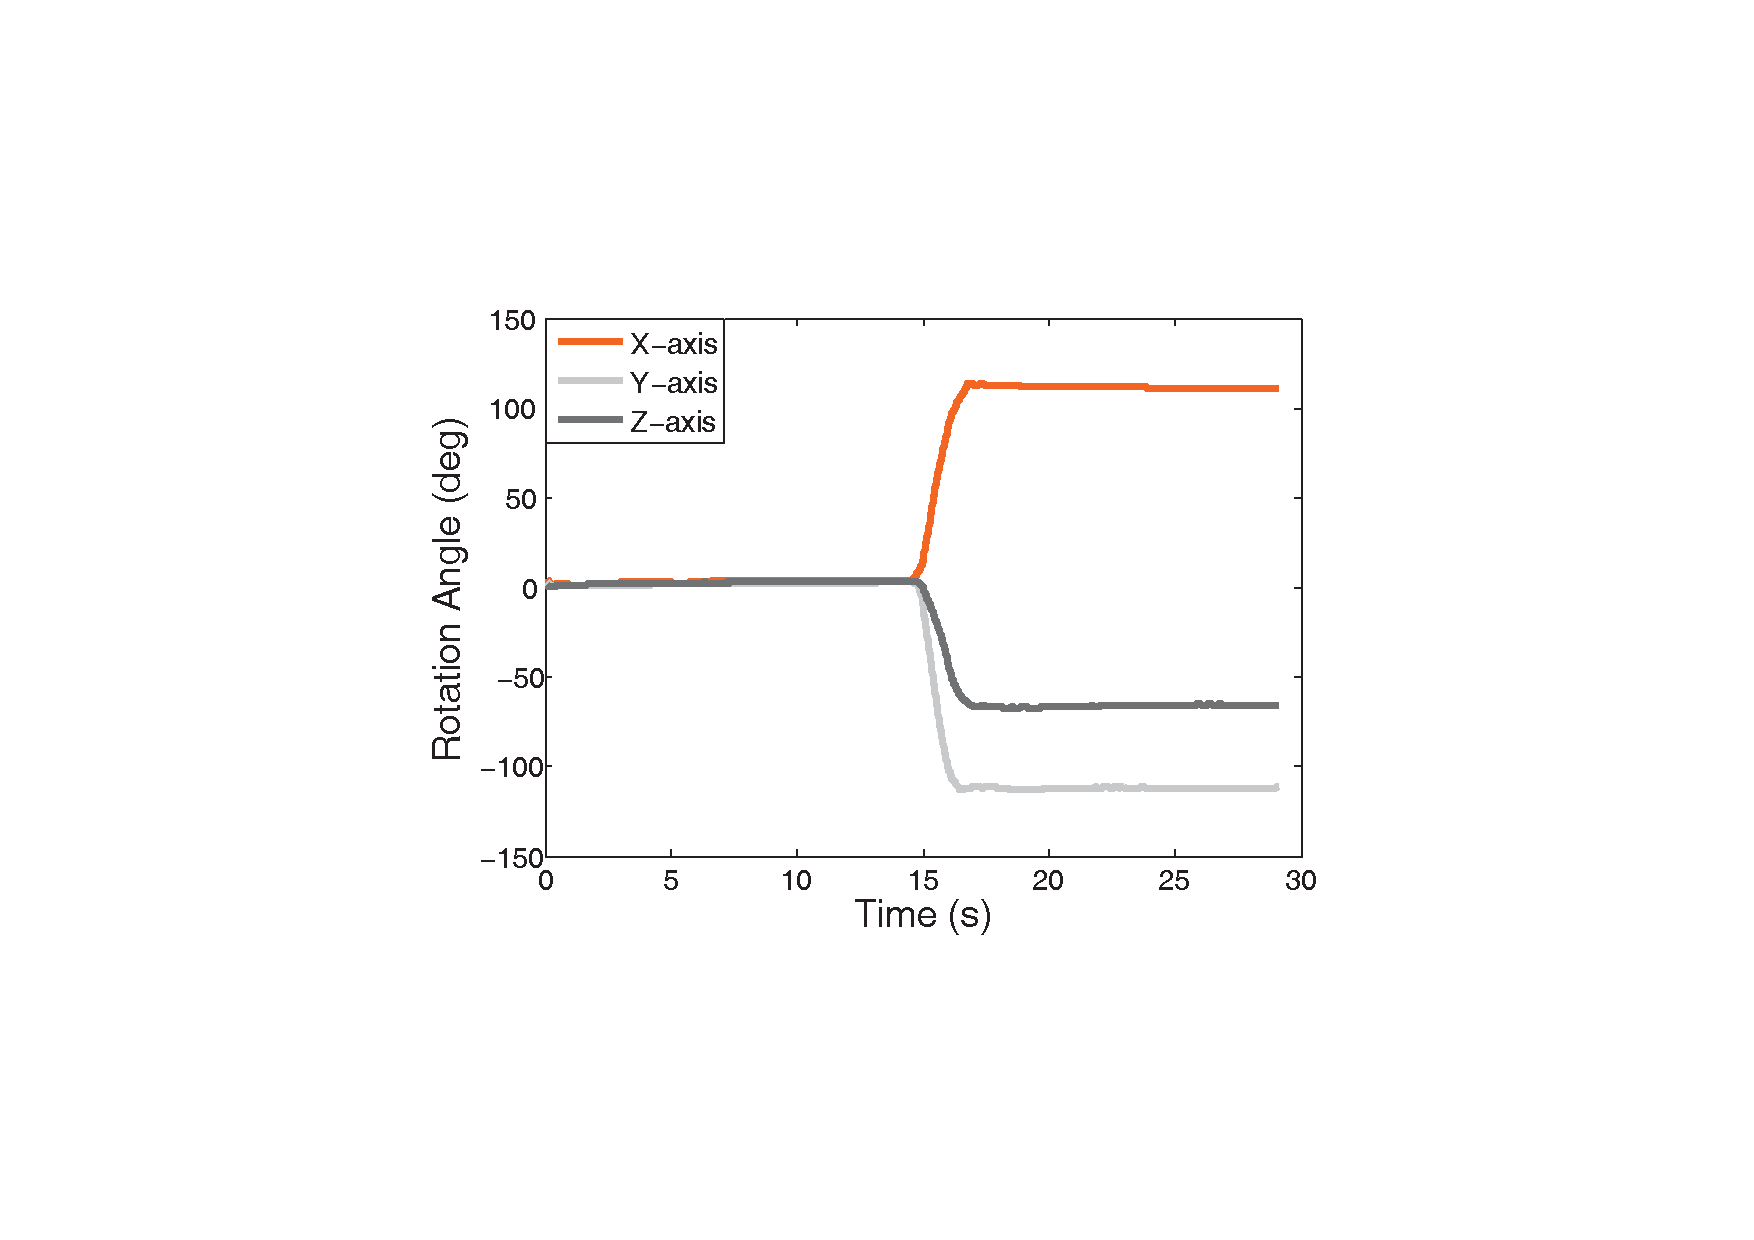
\includegraphics[width=0.32\linewidth]{Figures/BodytoHead.pdf}}
	\subfigure[moving to the abdomen]{\label{BodytoAbdomen}
		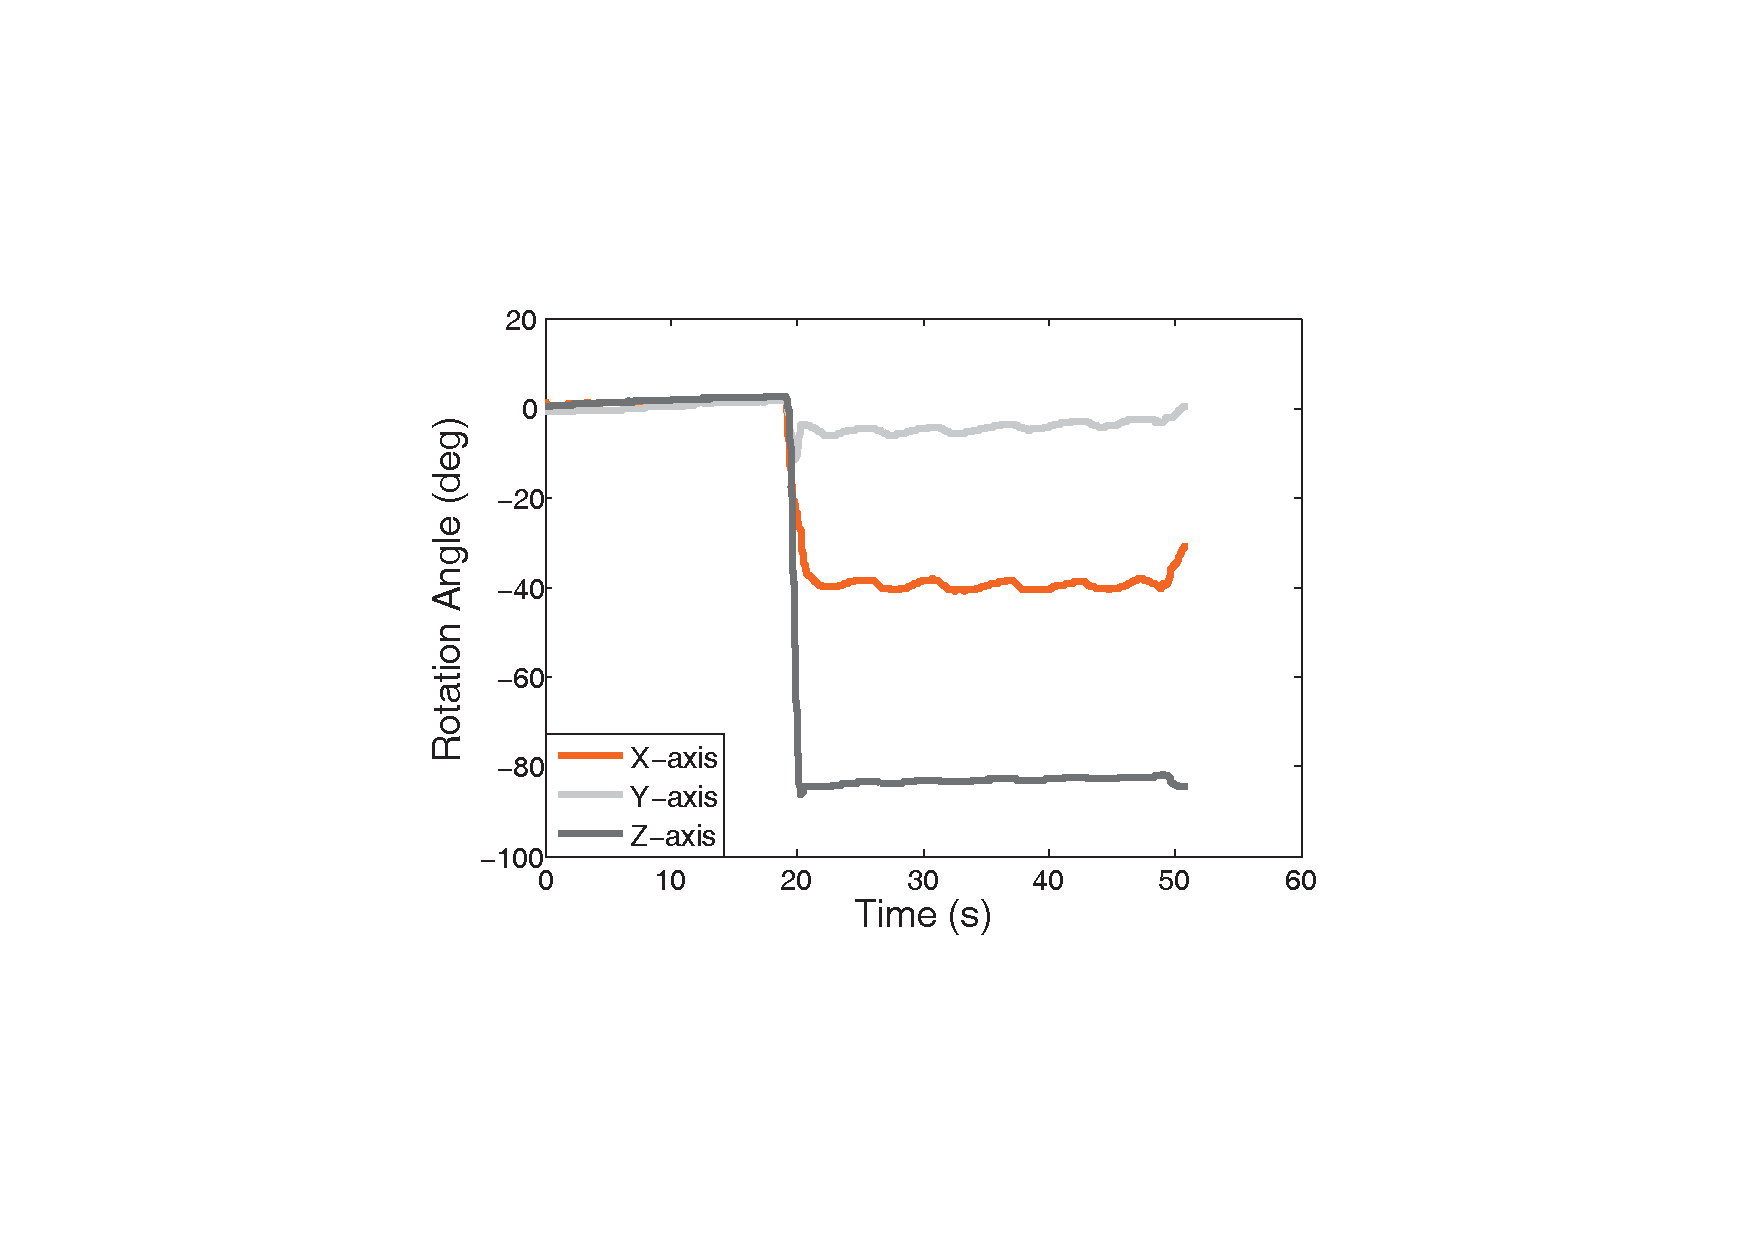
\includegraphics[width=0.32\linewidth]{Figures/BodytoAbdomen.pdf}}
	%  \hfill
	\subfigure[moving to the chest]{\label{BodytoChest}
		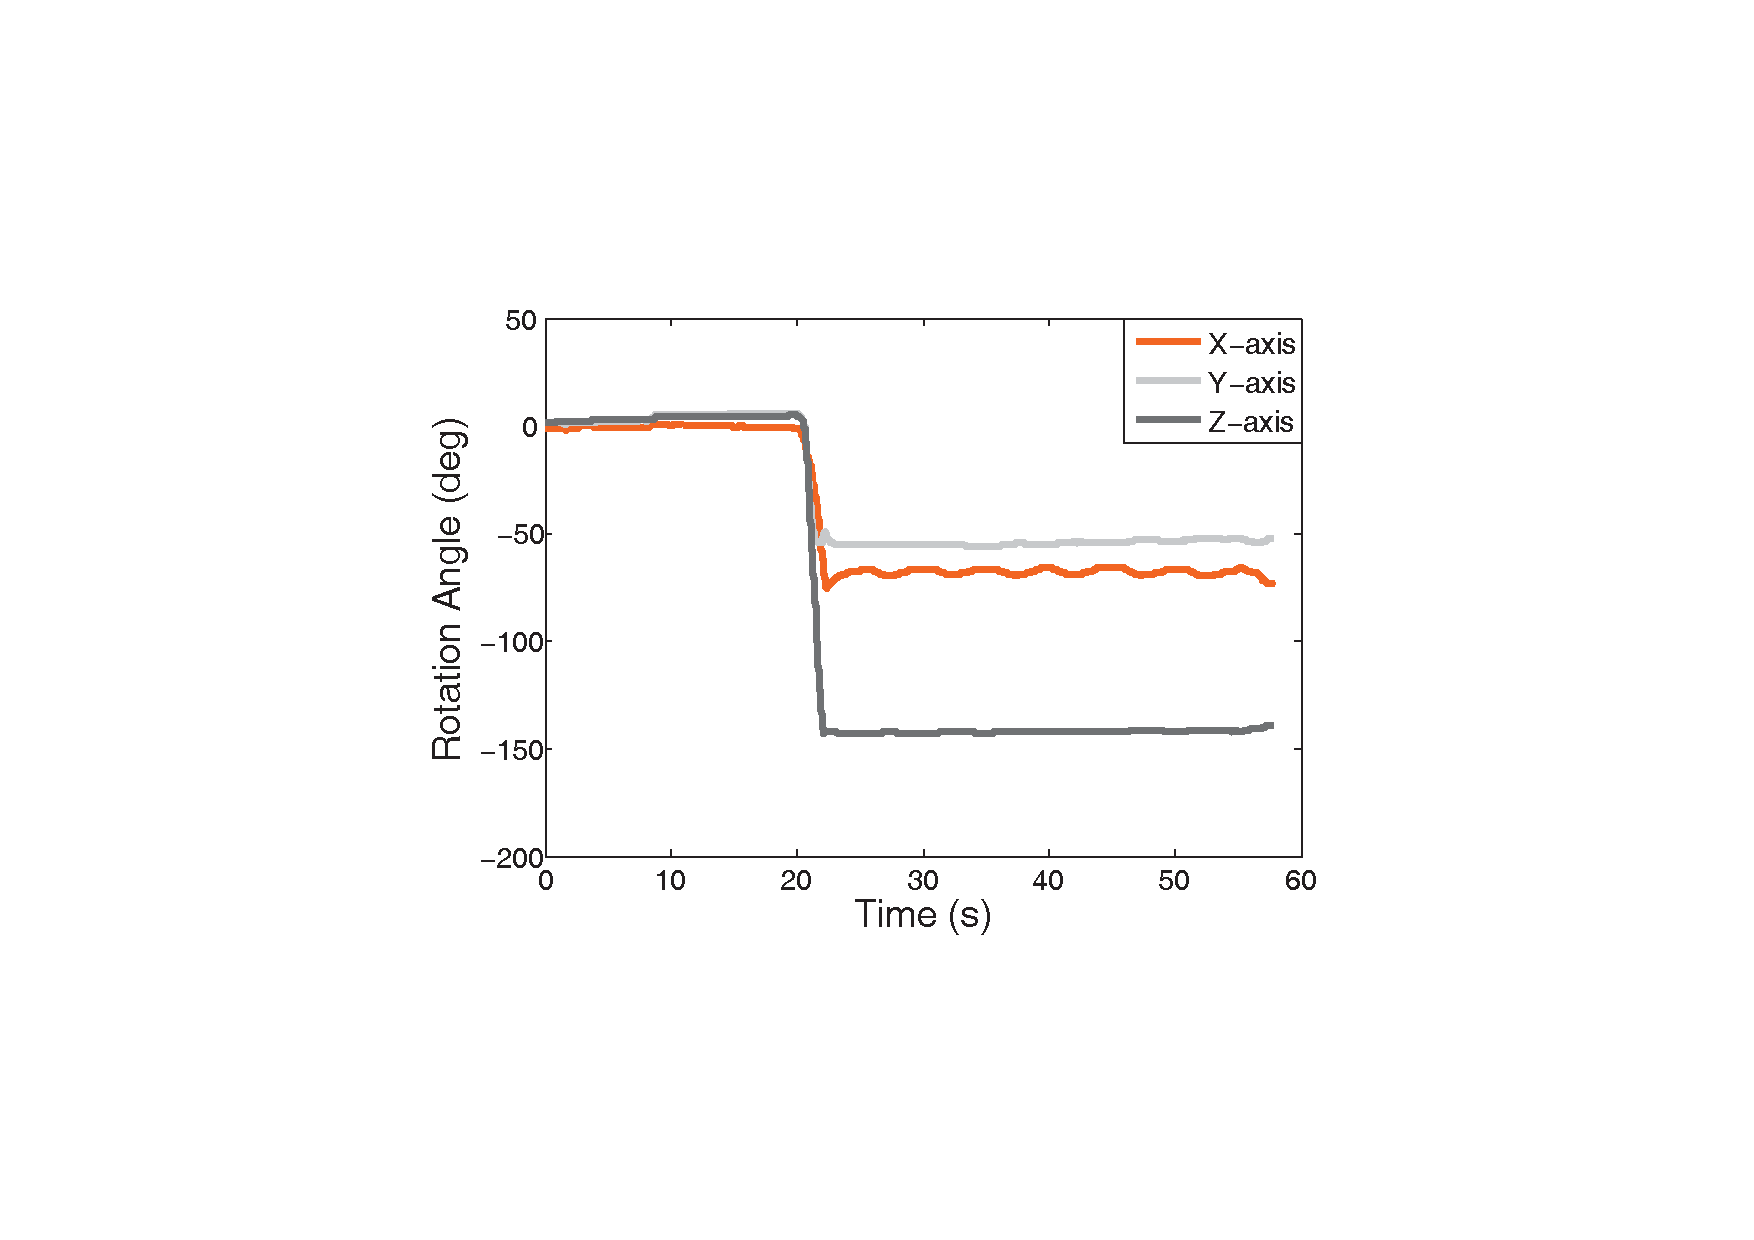
\includegraphics[width=0.32\linewidth]{Figures/BodytoChest.pdf}}
	%  \hfill
  %  \subfigure[moving to the shoulder]{\label{BodytoShoulder}
%		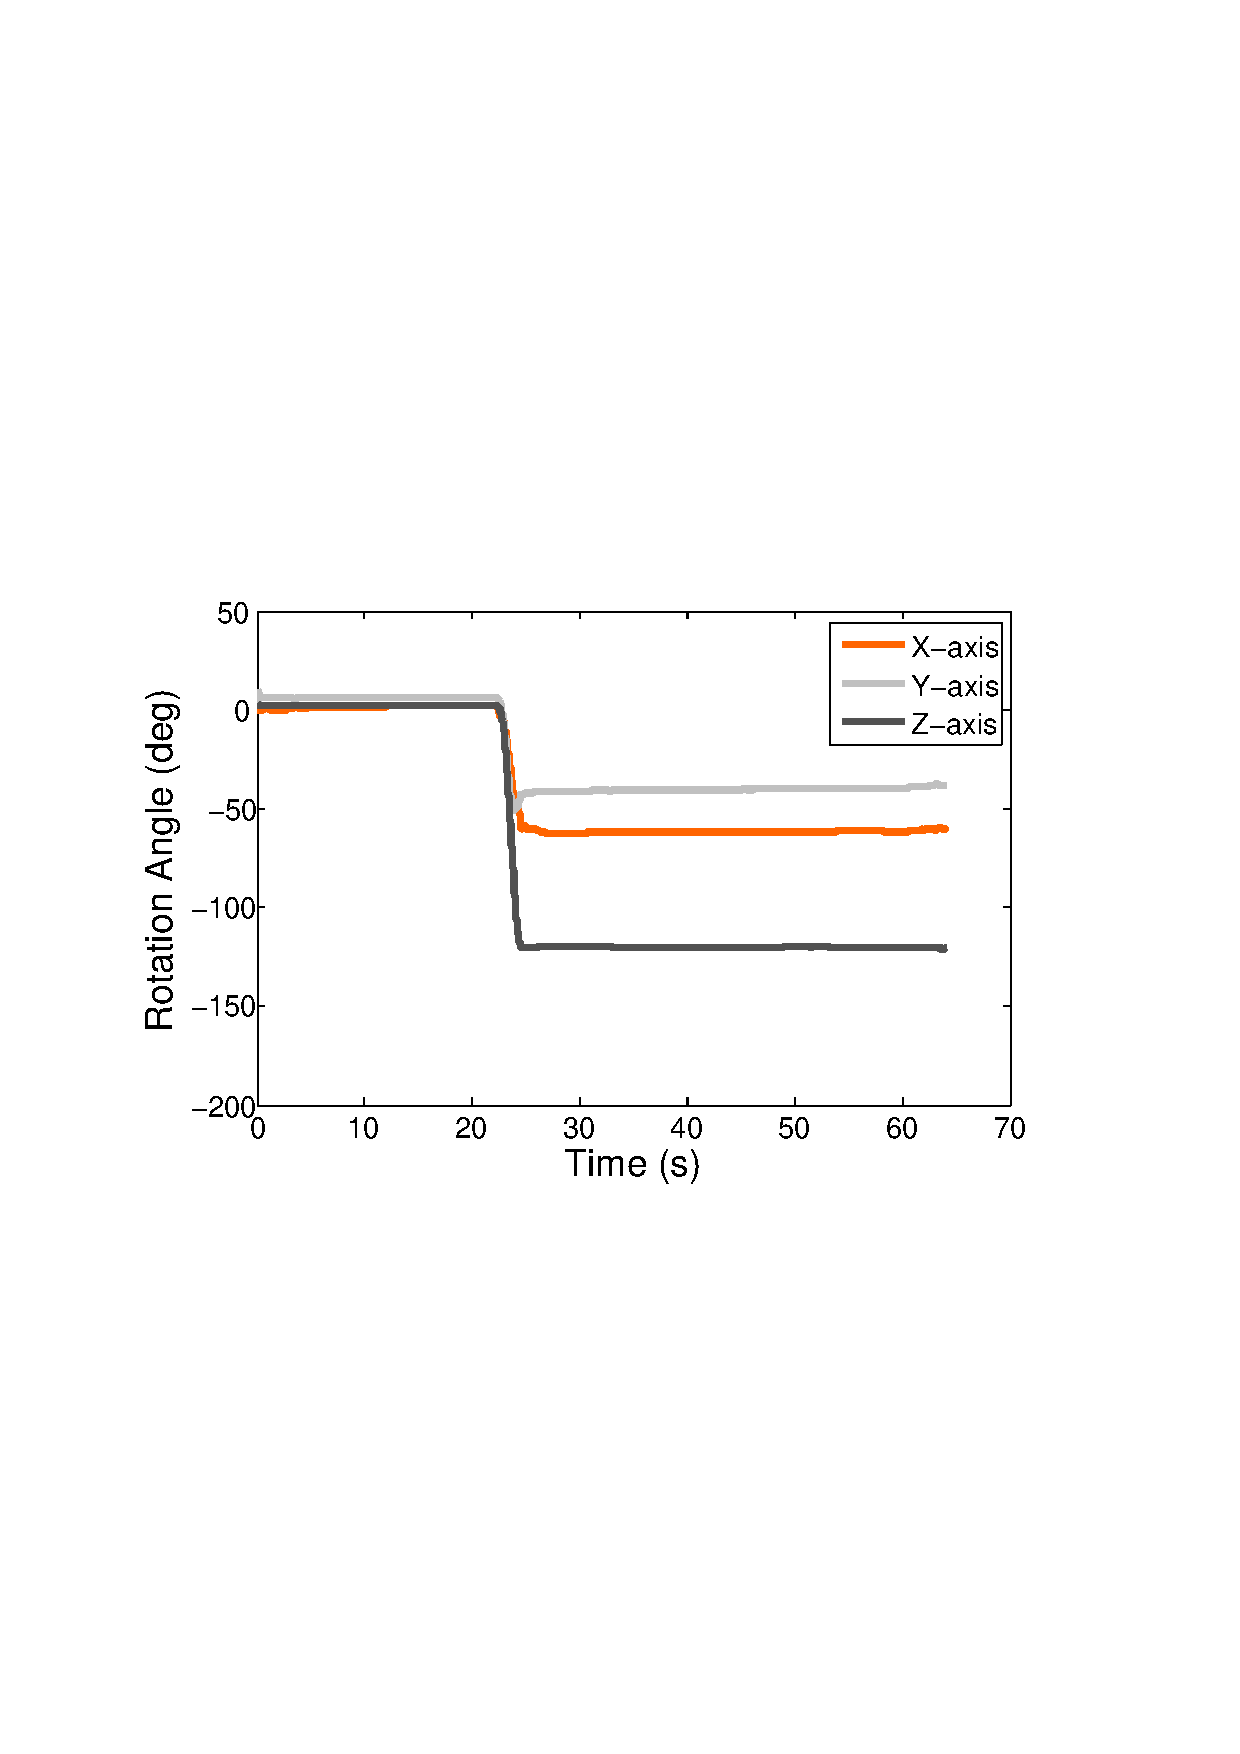
\includegraphics[width=0.34\linewidth]{Figures/BodytoShoulder.pdf}}
	\caption{The differences of the rotation angle when a hand of one of our users, placed next to the subject's body, is moved to his head (a), abdomen (b), and chest (c). }\label{Bodyhand}
\end{figure}

\begin{figure}
	\centering
	\begin{minipage}[t]{.475\textwidth}
	\centering
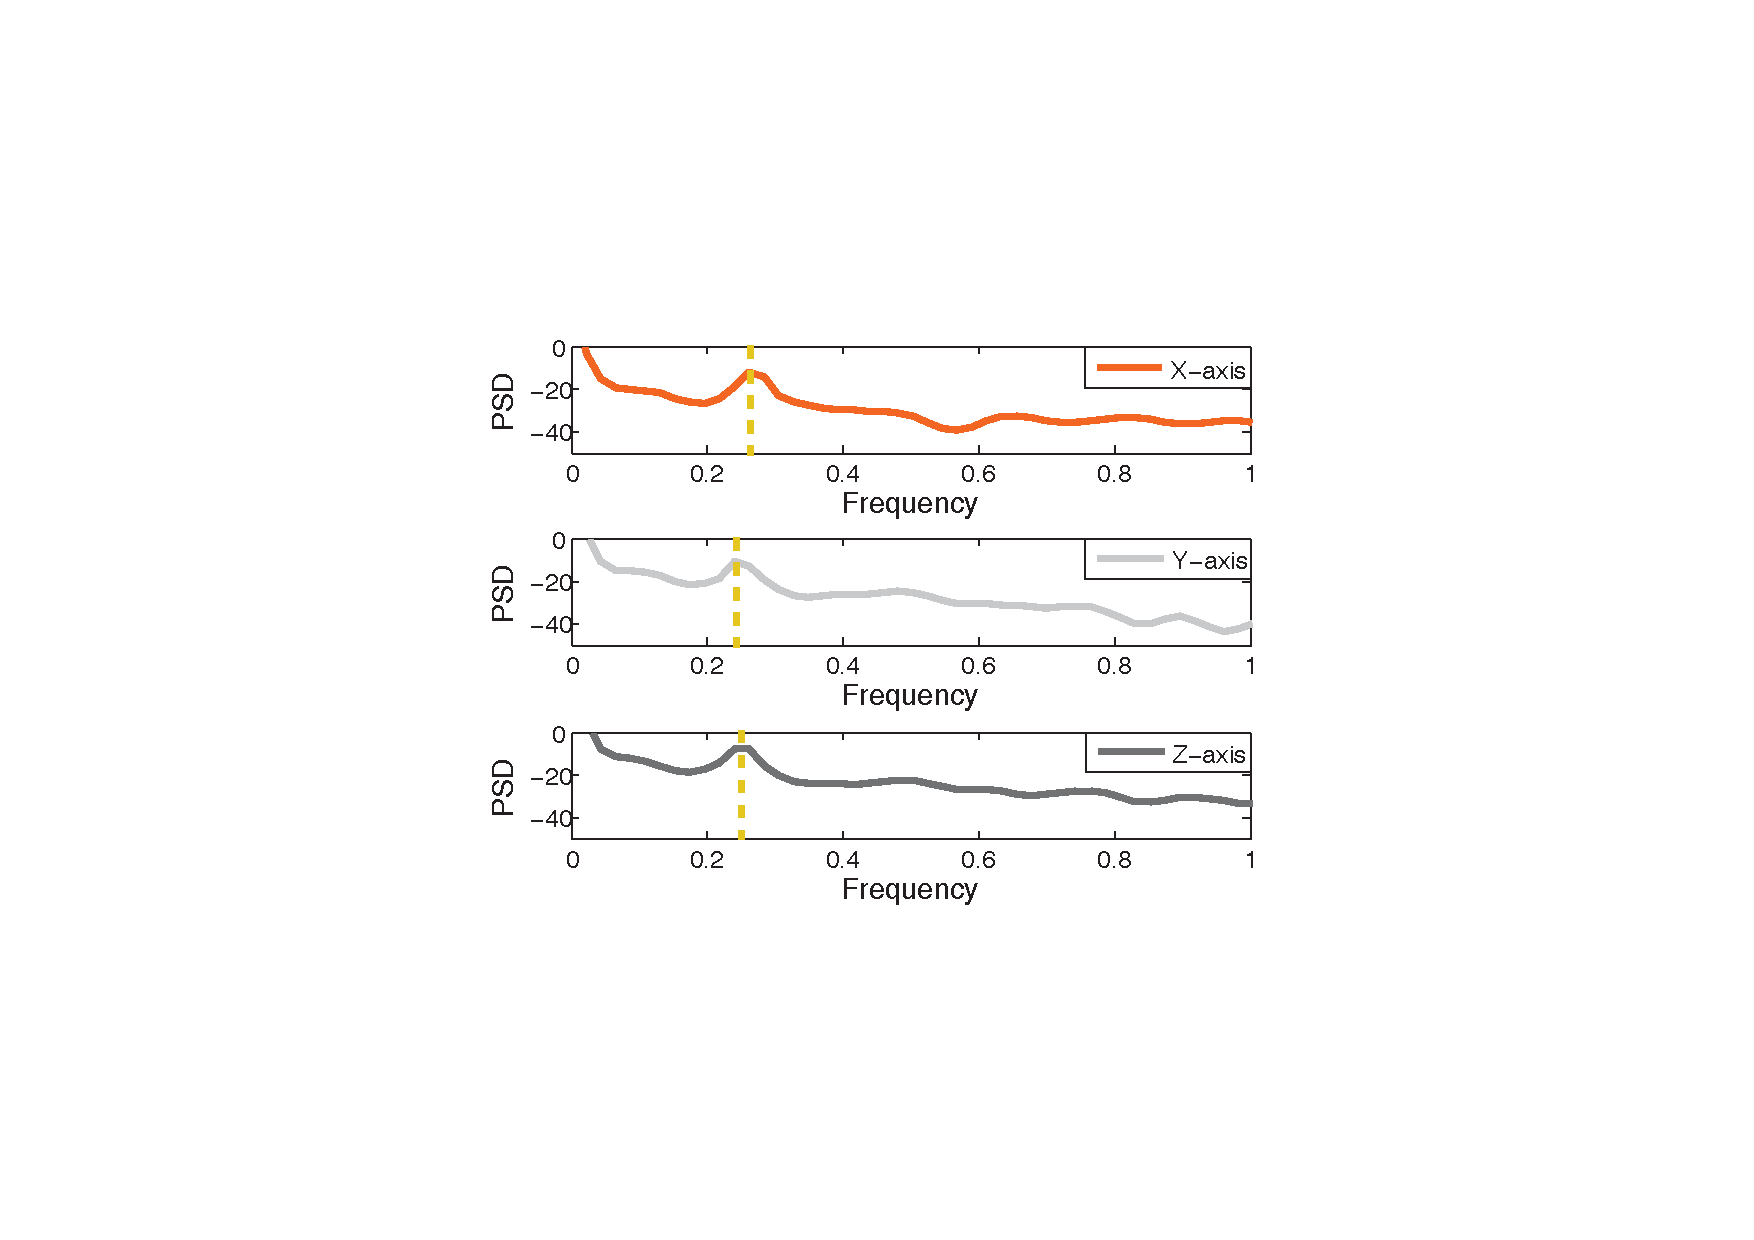
\includegraphics[width=7cm,height=5cm]{Figures/PSD.pdf}
\caption{The power spectral density (PSD) of the accelerometer readings when a user's hand is placed on his chest.}\label{fig:PSD}
	\end{minipage}%
\hfill
	\begin{minipage}[t]{.475\textwidth}
	\centering
	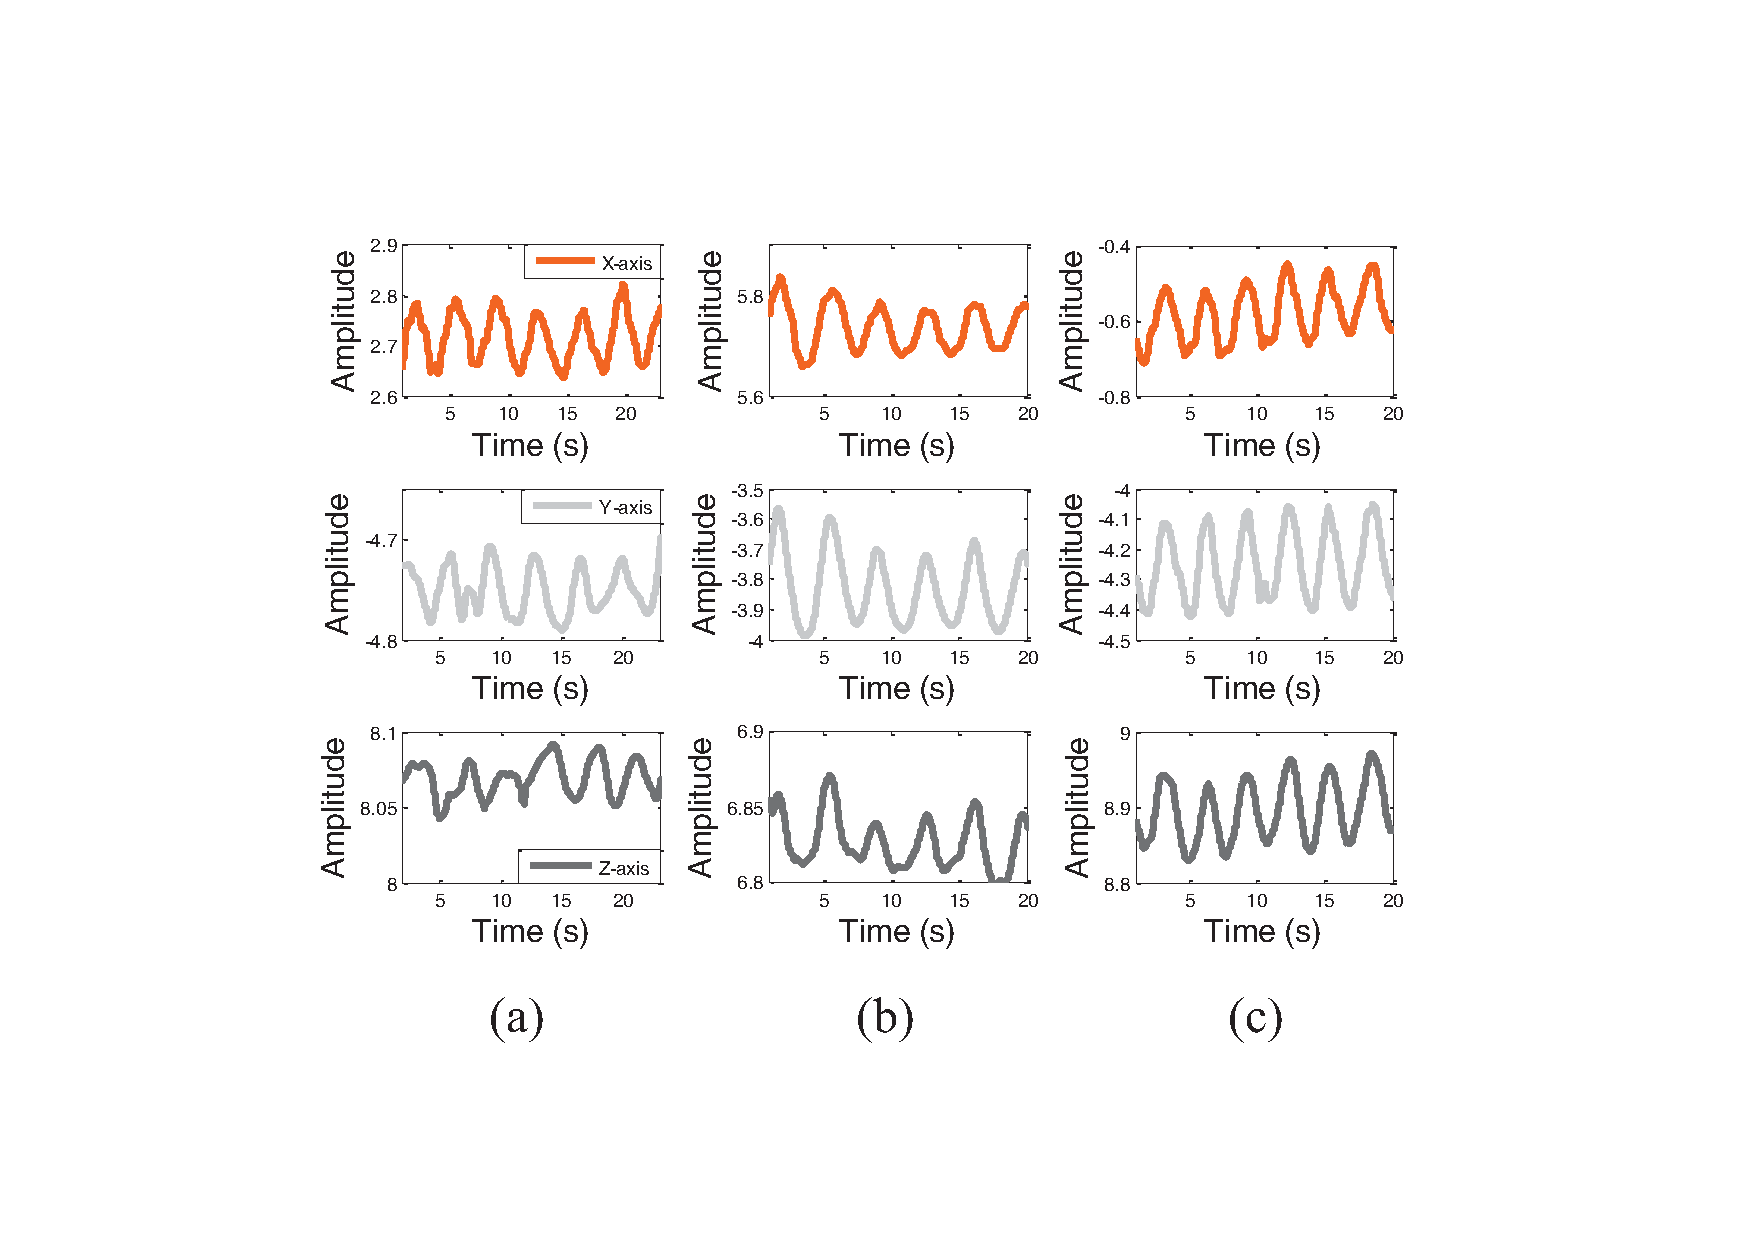
\includegraphics[width=7cm,height=5cm]{Figures/breath_ok1.pdf}
	\caption{The periodic change of the acceleration signal. (a) REM--Location 1. (b) REM--Location 2.  (c) NREM--Location 1.}\label{fig:breath_ok1}
	\end{minipage}
\end{figure}

%result in uniquely identifiable trajectories that are specified by the start and end point of the hand. By comparing information about the latest trajectory against movement templates (analogously to

%that we can identify current hand position by analysing the latest hand trajectory which caused the hand position to change. we have developed a novel algorithm that is based on the key intuition that, before the hand is placed on the body, it experiences a movement from side of the body to the end position, and after that the hand always experiences a movement from one position to the other. Thus we can further integrate the hand movement trajectory to determine the hand position at current time. In {\systemname}, We consider nine kinds of the trajectories of hand, from the side of the body to the abdomen, to the chest, to the head; from the chest to the abdomen, to the head; from the abdomen to the chest, to the head; from the head to the abdomen, to the chest.
%Fig.~\ref{Bodyhand} shows the rotation angle changes in three dimensions (x, y and z), when the hand next to the body is moved to different
%parts of the body. The data are collected using the gyroscope. To aid clarity, we present the data collected from one of the users
%participated in our pilot study, similar behaviors are observed for all other participants. \textcolor{blue}{In the picture, we only show
%the signals from a single subject. This is because after experiments we found that the three hand trajectories of the hand are roughly the
%same in different people. We only show the approximate relative trend to indicate that the difference in the hand trajectory. So we can use
%the three-axis rotation angle calculated by the gyroscope as a feature to establish a sample library, and use the template distance
%matching classifier to identify the final position of the hand. However, if we only use the hand's movement trajectory to determine the
%position of the hand, then we only get the movement relative to a certain known starting position, not the final absolute position of the
%hand. That is, only when we know that each time the starting position of the hand before movement, we can judge the final hand position
%based on different trajectories. However, in practical applications, it is difficult for us to obtain the starting position of the hand
%every time. Therefore, we only cannot rely on the hand movement trajectory to achieve the purpose of detection. However, we found that when
%the hand is placed on the head, the hand placement is clearly different from that of the hand on the chest or abdomen, which makes it
%easier to detect by the angle characteristics calculated by the acceleration when placed on the head. When the hand is on the chest or
%abdomen, the angle characteristics are very similar and difficult to distinguish. Hence, we need an additional verification step to ensure
%the hand is on the chest or abdomen. We can based on key intuition is that we can observe acceleration signals to exhibit a distinctly
%periodic fluctuation, as shown in Fig. \ref{Bodyhand}. This is due to the movement of the abdomen and chest caused by breathing. Therefore,
%we can use the occurrence of respiratory events to determine if the hand is indeed on the body (abdomen or chest). Through the detection of
%respiratory events, we can not only determine the initial position of the hand before movement but also filter out some areas near the
%chest or abdomen, such as the shoulders or hips. This is because when the hand move to the shoulder or hip and some other areas close to
%the chest or abdomen, the resulting hand trajectories are very similar, but we can not observe significant respiratory events, as shown in
%Fig. \ref{BodytoChest} and Fig. \ref{BodytoShoulder}. So we can combine with the hand's movement trajectory to accurately determine the
%hand position.}

\paragraph{Detect the abdomen and the chest positions.}

If our hierarchical model predicts that the hand was not placed on the head, the hand could be located at anywhere including different
parts of the body. Recall that we are interested at detecting if the hand is placed on three positions: the head, the abdomen and the
chest. This means in addition to the head position model, we still need to find ways to detect if the hand was placed on the abdomen or the
chest. We found that the hand is likely to be affected by the breathing if it is placed on these two body locations. Specifically, the
 impact of breathing leads to periodical fluctuations on the accelerometer readings. This is because the hand will be pushed up and drop down because of
breathing when it is placed on the abdomen or the chest. Our experimental data suggest that this is a unique behavior that is only observed
when the hand is placed on the abdomen or the chest, but not other part of the body (such as the shoulder).


To examine if the accelerometer data are affected by the respiration because the hand is placed on the abdomen or the chest, we calculate
the power spectral density (PSD) of the collected accelerometer data. We then check if there is any peak value matches the human
respiratory frequency. A match indicates that the hand is affected by a respiratory event and hence the hand is likely to be placed on
either the abdomen or the chest. Fig. \ref{fig:PSD} provides an empirical evidence to support our design choice. It shows the PSG for one
of our pilot study user when his hand was placed on the chest. Here we calculate the PSD for the accelerometer data collected from the x, y
and z directions. We can see from the diagram that there is a large peak located at around 0.25Hz (highlighted in the diagrams) when a
respiratory event is detected (which is labeled by watching the video). This peak corresponds to the average respiratory frequency of an
adult (0.2Hz to 0.47Hz)~\cite{Breath_frequence}, suggesting that the PSD reading can be used as a proxy to detect respiratory events.
\systemname thus exploits the PSD to detect if the hand is placed on the abdomen or the chest by checking if there is any peak value of PSD
falls within the range of 0.2Hz (corresponding to 12 breathes per minute) and 0.47Hz (corresponding to 28 breathes per minute).

With the PSD-based method in place (which tells us if the hand is placed on the abdomen or the chest or elsewhere), we then use again a KNN
classifier to make a binary decision to determine if the hand is placed on the abdomen or the chest based on the rotation angle readings
(see Fig.~\ref{Bodyhand} b and c). Like the head position model, the training samples for the KNN model are also collected from our pilot
study users -- where each training example includes the rotation angle readings when the hand is either placed on the abdomen or the chest.

\subsection{Labeling the Eye Movement Stages}

We also found that the extent of body movements can be used to judge the amplitude of respiration, which in turns allows us to detect
rapid-eye-movement (REM) and non-rapid-eye-movement (NREM) stages. This is based on the prior study showing that when people sleep in the
REM stage, their respiratory amplitude is smaller than that in the other stages~\cite{respiratory1982}. Hence, we can roughly determine the
user's current sleep stage based on the respiratory amplitude. Respiratory amplitude is only an indicator of the division of the sleep
stage and we can not regard it as a basis for final judgement, but it serves as an early reference that helps later phases of the sleep
stage detection. Under normal circumstances, the chest movement amplitude is smaller than abdominal movement amplitude. However, in
different sleep stages, the respiration amplitudes are different~\cite{respiratory}. It is likely that there is a situation: the chest
movement amplitude in the NREM stages is close to the abdominal movement amplitude in the REM sleep stage. As a result, the threshold based
method cannot work. At this time, we need to combine it with the position of the hand we detected with the trajectory before. Through the
above steps, we have been able to determine whether the hands are on the chest or abdomen, and then we can go further to determine the
extent of breathing according to the degree of body ups and downs, and we can roughly infer the sleep stage. Now we take the case of hands
on the abdomen as an example.



    Even when the hand is placed on the abdomen, due to minor changes in the exact location of the user's hand, the location of intensity of
accelerometer fluctuations caused by respiration varies. Hence, we cannot use the amplitude information to determine true respiratory
amplitude directly. This problem is illustrated in Fig.~\ref{fig:breath_ok1}, where (a) and (b) contain triaxial acceleration measurements
at different locations of the abdomen during REM sleep stage, and in (c) which consists of acceleration data for NREM stages at the same
approximate position as in (a). We can see that when hand on the abdomen, but the location is different, even in the same location, we can
not directly judge the respiration amplitude using only the amplitude of the three axes of the acceleration.

\begin{figure}[!t]
\centering
      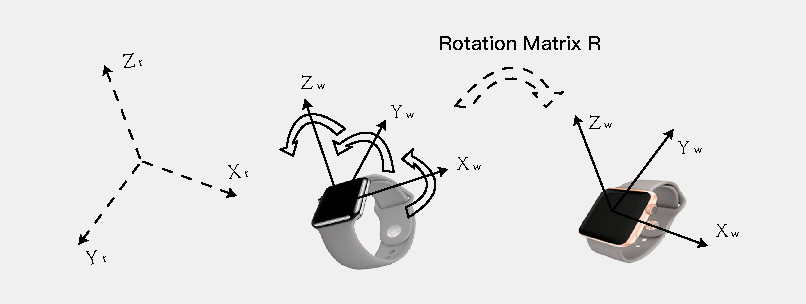
\includegraphics[width=0.67\linewidth]{Figures/watch.pdf}
  \caption{The first figure on the left is the torso coordinate system, and $Y_t$ points north. The middle figure shows the watch coordinate system when the watch an arbitrary position, and the right of the figure shows that the  watch coordinate system after we completed the coordinate system conversion.}\label{fig:watch}
\end{figure}

To solve this problem, we convert the acceleration data from the wristwatch coordinate system into the data in the torso coordinate system. Because we can know that when the person is in the supine position, the abdomen and the chest will move up and down due to breathing, that is, move along the z-axis direction of the torso coordinate system. We express the triaxial acceleration data as $Acc_w$ = [$X_w$, $Y_w$, $Z_w$] in the wristwatch coordinate system and $Acc_t$ = [$X_t$, $Y_t$, $Z_t$] in the torso coordinate system, as shown in Fig. \ref{fig:watch}. And the watch coordinate system ({[$X_w$, $Y_w$, $Z_w$]}) is determined by the position of the watch. Our coordinate alignment aims to find a rotation matrix R to align the watch's coordinate system to the torso coordinate system ({[$X_t$, $Y_t$, $Z_t$]}) and R can be obtained by the three-axis direction information in the orientation sensor. After the coordinate system is aligned, the angle between the y-axis of the wristwatch coordinate system and the y-axis of the torso coordinate system is 180 degrees.
\begin{equation}
      X_t  = (X_w {\cos\gamma} + Y_w{\sin\gamma}){\cos\theta} + (Y_w\cos\sigma + Y_w\sin\sigma)\sin\theta,
\end{equation}
\begin{equation}
      Y_t = -((Y_w\cos\sigma + Y_w\sin\sigma)\cos\theta - (X_w\cos\gamma + Y_w\sin\gamma)\sin\theta),
\end{equation}
\begin{equation}
      Z_t = (Z_w\cos\gamma - Z_w\sin\gamma)\cos\sigma - (Z_w\cos\gamma - Z_w\sin\gamma)\sin\sigma,
\end{equation}

$\theta$, $\sigma$ and $\gamma$ are the x, y and z axis data of the orientation sensor respectively, representing the direction angle, the tilt angle and the roll angle collected from the orientation sensor. After the alignment of the coordinate system, we can see from Fig.~\ref{fig:cordi} that the z-axis shows a periodic signal with significant fluctuations, while the x- and y-axis data undergo smaller changes around zero, which is consistent with the actual situation that when the person is in the supine posture with the abdomen up and down caused by respiratory.

 \begin{figure}[!t]
\centering
      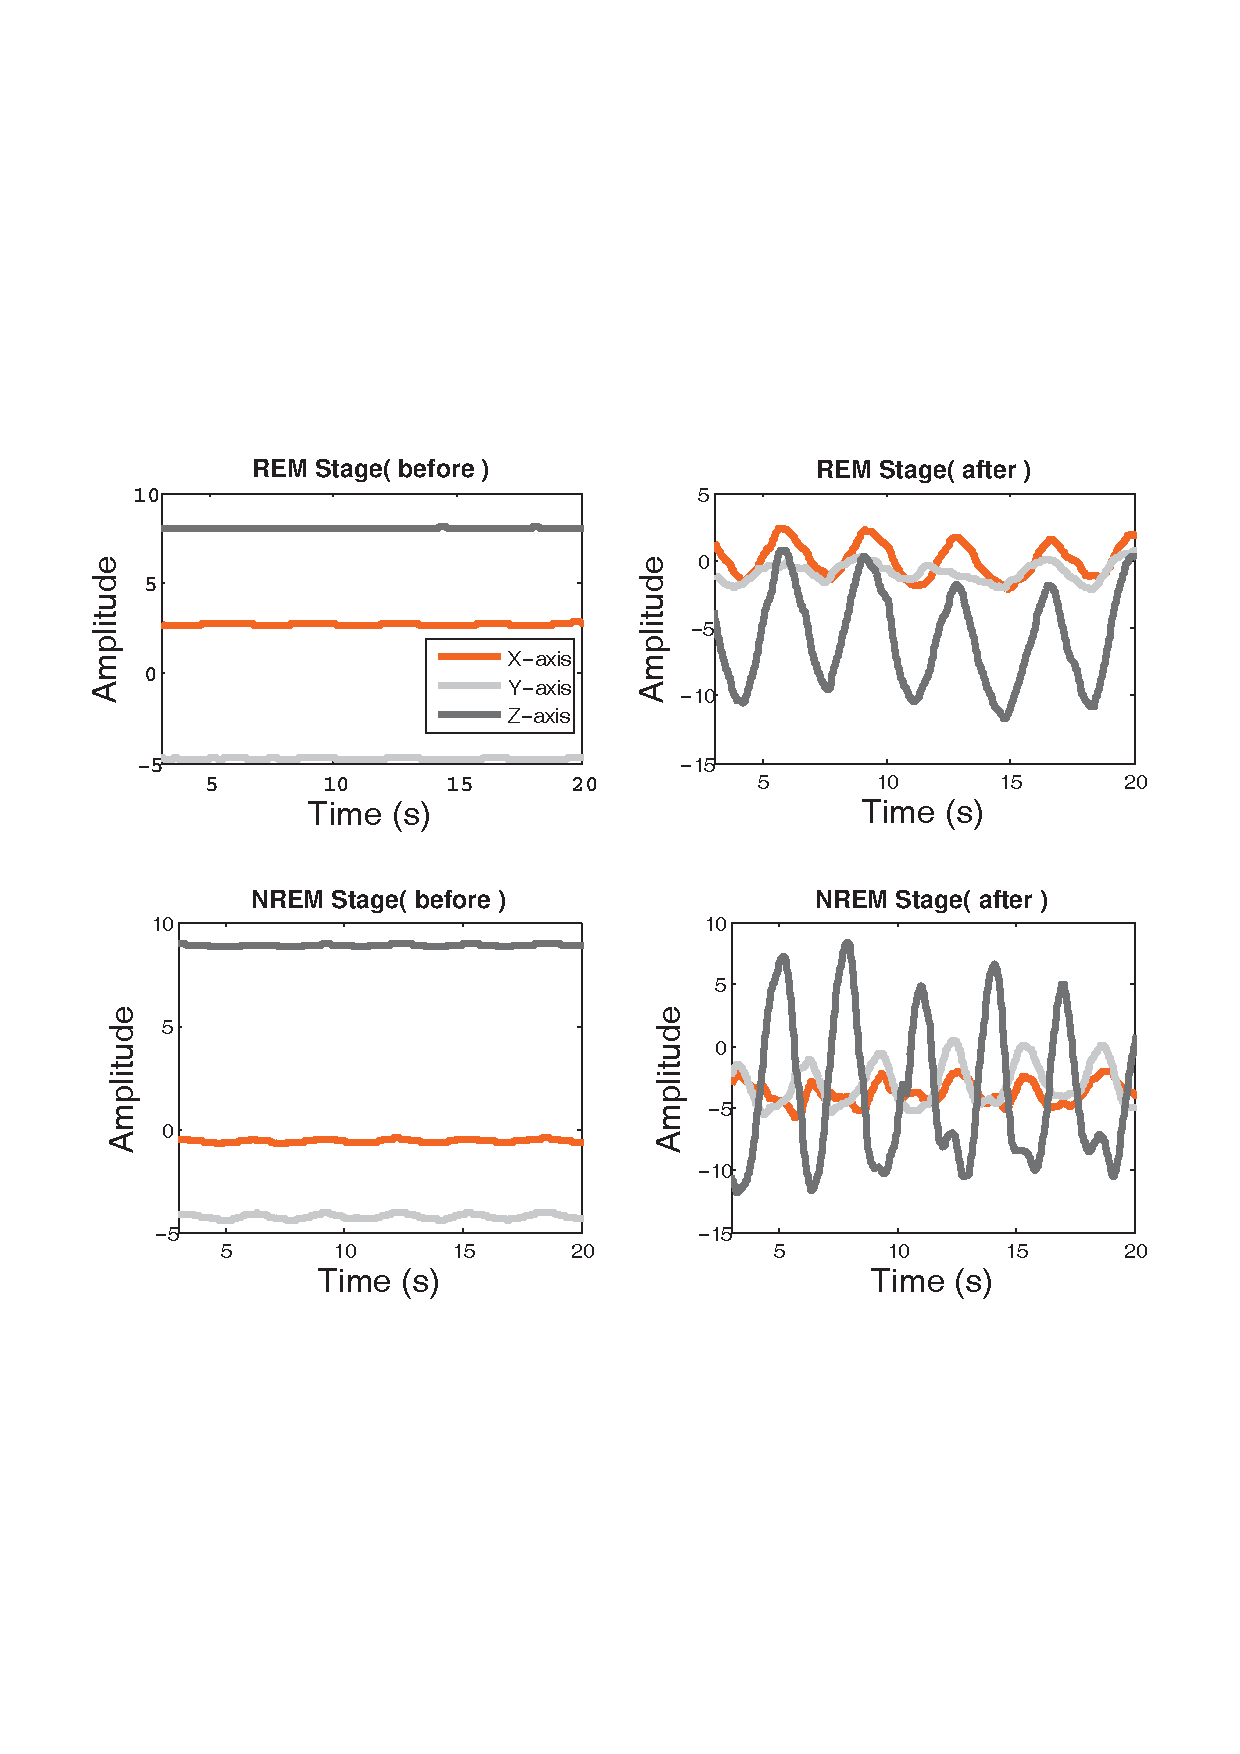
\includegraphics[width=0.75\linewidth]{Figures/cordi.pdf}
  \caption{Acceleration data for different sleep stages.}\label{fig:cordi}
\end{figure}

The two graphs on the left of Fig.~\ref{fig:cordi} show the same acceleration data as has been used in (a) and (c) of
Fig.~\ref{fig:breath_ok1}, respectively, whereas the two right-most graphs correspond to the data after coordinate system alignment.  We
can see that prior to align the measurements, we cannot effectively distinguish the respiratory amplitude of REM and NREM stages from the
acceleration amplitude. After coordinate alignment, the respiratory amplitudes are clearly visible from the z-axis data. We then calculate
the variance of z-axis acceleration and use it as a feature to measure the intensity of the fluctuation in a signal, with larger variance
corresponding to greater breath amplitude. Note that we cannot use the sum or magnitude of the z-axis as a measure of intensity as the
measurements remain affected by gravity.

\textcolor{cyan}{ We use the respiratory amplitude to detect whether the user is at the REM or not. Specifically, we calculate the
respiratory amplitude when the hand is found to be placed on the abdomen or the chest (\systemname can only detect respiratory events when
the hand is placed one of these two positions). We then use a KNN classifier to find from our training examples, which training example is
most similar to the input respiratory amplitudes collected from the x, y, and z directions. The similarity is measured by calculating the
Euclidean distance on the 3-dimensional feature space. We then use the label (either REM or NREM) associated with the nearest training
example as the classification outcome.}

\textcolor{cyan}{ To generate the training examples, we first use our hand position recognition algorithm described in
Section~\ref{sec:handpr} to detect, from our training dataset (see (Section~\ref{sec:trainingdata}), wheter the hand was placed on the
abdomen or the chest to calculate the respiratory amplitude. We can consider the user is at either (1) the NREM stage if a large repository
amplitude (i.e., the amplitude value is not less than 15) is detected, or (2) the REM stage if a normal repository amplitude (i.e., the
amplitude value is not greater than 4) is detected. These thresholds are chosen based on prior study\FIXME{ \cite{}}. To remove the noises
of the training data, we only use training examples where both our approach and Fitbit reach the consensus on the eye movement stage. We
also manually inspect the recorded videos to label the stage from our training data.}



%\textcolor{blue}{We then trained a classifier based k-nearest neighbor model (with k = 1) using this feature when the hand is placed on the
%abdomen and on the chest under both REM stage and NREM stages to determine a mapping from current respiratory amplitude to placement. Here,
%we define the respiratory amplitude in the NREM stage as large respiratory amplitude, and the respiratory amplitude in the REM stage as
%normal respiratory amplitude. As for the acquisition of sleep stage, we confirm the label of it when both Fitbit and {\systemname} reach a
%consensus. At the same time, We also take into account video recorded by the camera to manually label part of the respiratory. The
%combination of these three kinds of equipment can enable us to obtain real and accurate data as much as possible.  As classifier we used a
%decision stump which was trained on 200 sets of acceleration data (100 sets of these from the larger respiratory amplitude and the rest of
%sets from the normal respiratory amplitude ) from 10 volunteers, who are randomly recruited by us aged 16 to 60 years old.  The resulting
%threshold for the acceleration variance is around 15 when the hand on the abdomen, and around 4 when the hand is placed on the chest.}
%


\subsubsection{Body rollover counts \label{sec:bodyrollover}}

Under normal circumstances, people usually rollover their body around 20-45 times a night. The main function of body rollovers is simply to
maintain a comfortable sleeping position as maintaining the same position for prolonged period will result in muscular tension due to
hindered blood supply, which can also lead to local numbness~\cite{rollover2014}. So body rollover is another key indicator about the sleep
quality. {\systemname} can detect the number of body rollovers, which can get some reflections of sleep status and the roll-over frequency
can also help us to classify the sleep stage~\cite{rollover2007}. In general, there are six cases: four posture transition cases between
the supine posture and lateral (left or right) posture, and two posture transitions between the left lateral posture and right lateral
posture. Fig. \ref{fig:BodyRollover} shows the case when the body moves from the left side to the right side.
%
\textcolor{cyan}{The most intuitive way for detecting body rollover events is to estimate the rotation direction of the arm based on the
rotation angle given by the gyroscope. However, doing so is non-trivial because different users can exhibit drastically different patterns
for arm rotations; and the subtle changes in the starting arm position for the same sleeping posture could lead to a misprediction. As an
alternative to the rotation angle, we find that the tilt angles to be useful for this task because they strongly correlate to a body
rollover event. This correlation thus enables us to effectively translate the change of the tilt angle to a body rollover event to count
the occurrence of such events.} Specifically, the angle values of three different axes are on the falling edge or rising edge
simultaneously during a very short time period. Fig. \ref{fig:LeftToRight} -- Fig. \ref{fig:RightToLeft} shows the value changes under
different body rollover cases. To this end, a naive method to detect rollovers would be to rely on changes in angle measurements. However,
this method suffers a very large error since other hand movements will also induce a similar change.

\begin{figure*}[!t]
%\centering
%   \setlength{\abovecaptionskip}{-2pt}
% \setlength{\belowcaptionskip}{-9pt}
\begin{minipage}[t]{0.31\linewidth}\centering
    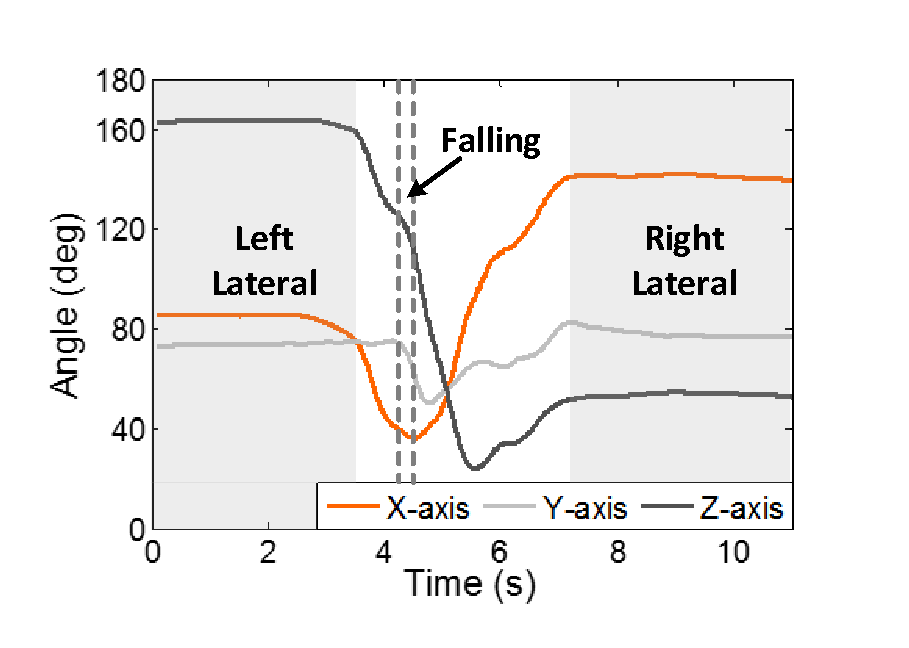
\includegraphics[width=0.97\linewidth]{Figures/LeftToRight.pdf}\centering
  \caption{From left lateral posture to right lateral posture.}\label{fig:LeftToRight}
\end{minipage}
\hspace{2pt}
\begin{minipage}[t]{0.31\linewidth}\centering
    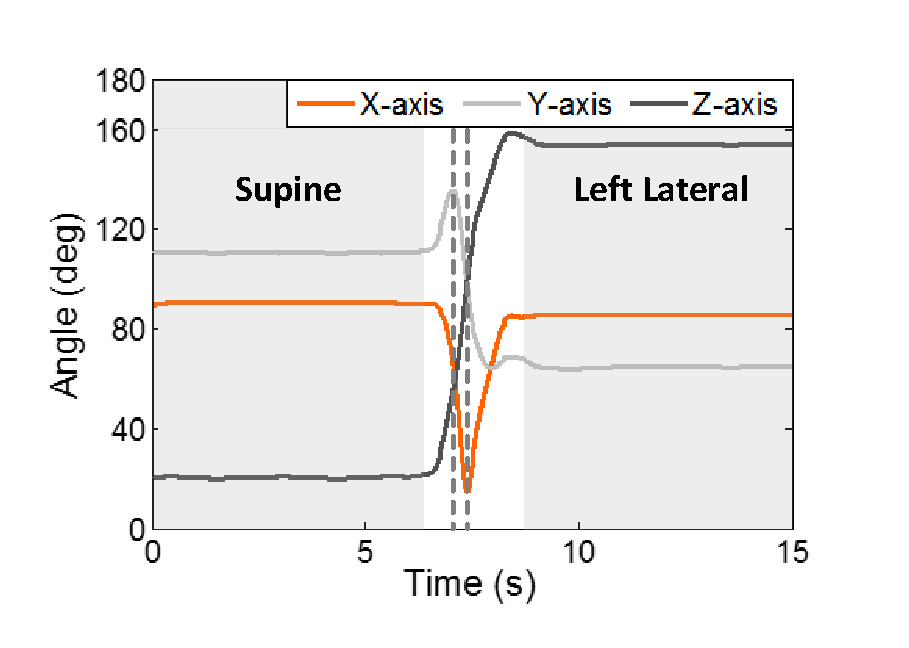
\includegraphics[width=0.97\linewidth]{Figures/SupineToLeft.pdf}\centering
  \caption{From supine posture to left lateral posture.}\label{fig:SupineToLeft}
\end{minipage}
\hspace{2pt}
\begin{minipage}[t]{0.31\linewidth}\centering
    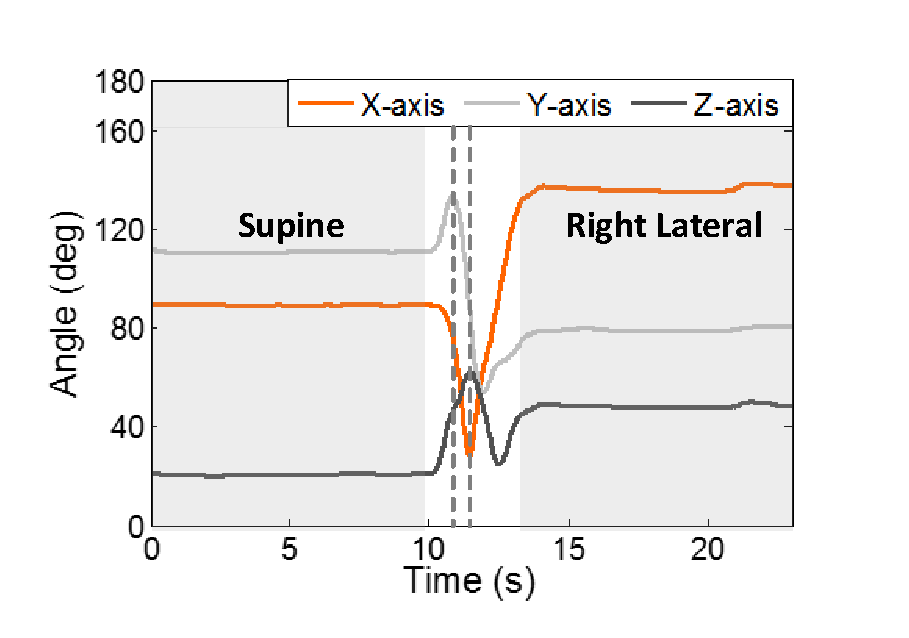
\includegraphics[width=0.97\linewidth]{Figures/SupineToRight.pdf}
  \caption{From supine posture to right lateral posture.}\label{fig:SupineToRight}
\end{minipage}
\end{figure*}

\begin{figure*}[!t]
\begin{minipage}[t]{0.31\linewidth}\centering
    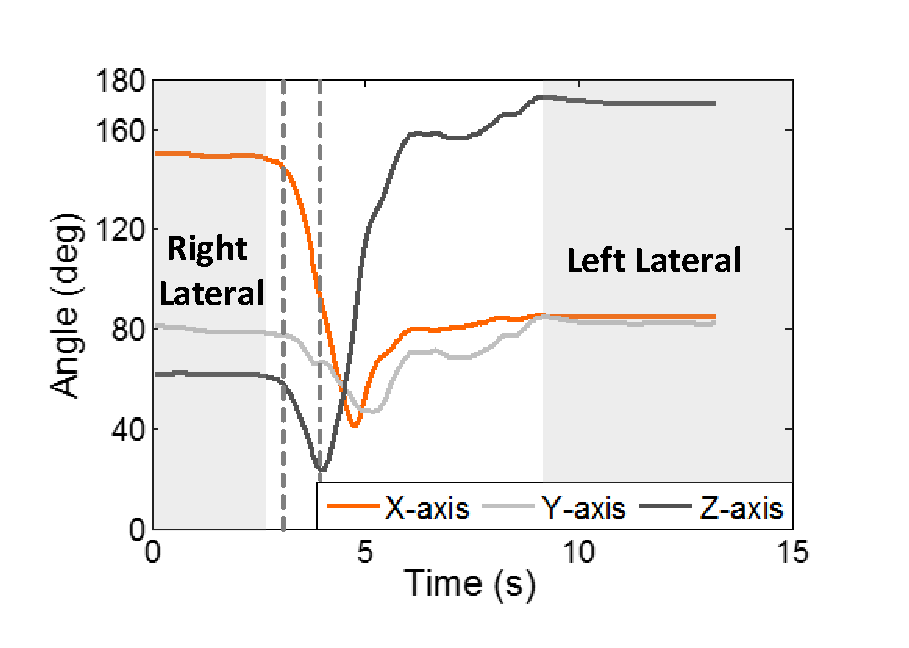
\includegraphics[width=0.97\linewidth]{Figures/RightToLeft.pdf}
  \caption{From right lateral posture to left lateral posture.}\label{fig:RightToLeft}
\end{minipage}
\hspace{2pt}
\begin{minipage}[t]{0.31\linewidth}\centering
    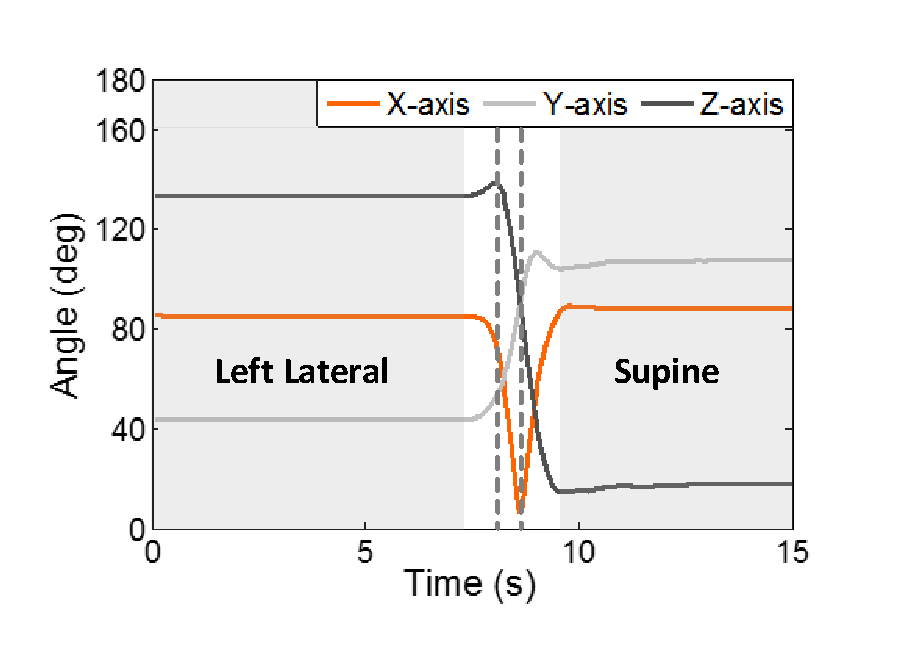
\includegraphics[width=0.97\linewidth]{Figures/LeftToSupine.pdf}
  \caption{From  left lateral posture to supine posture.}\label{fig:LeftToSupine}
\end{minipage}
\hspace{2pt}
\begin{minipage}[t]{0.31\linewidth}\centering
    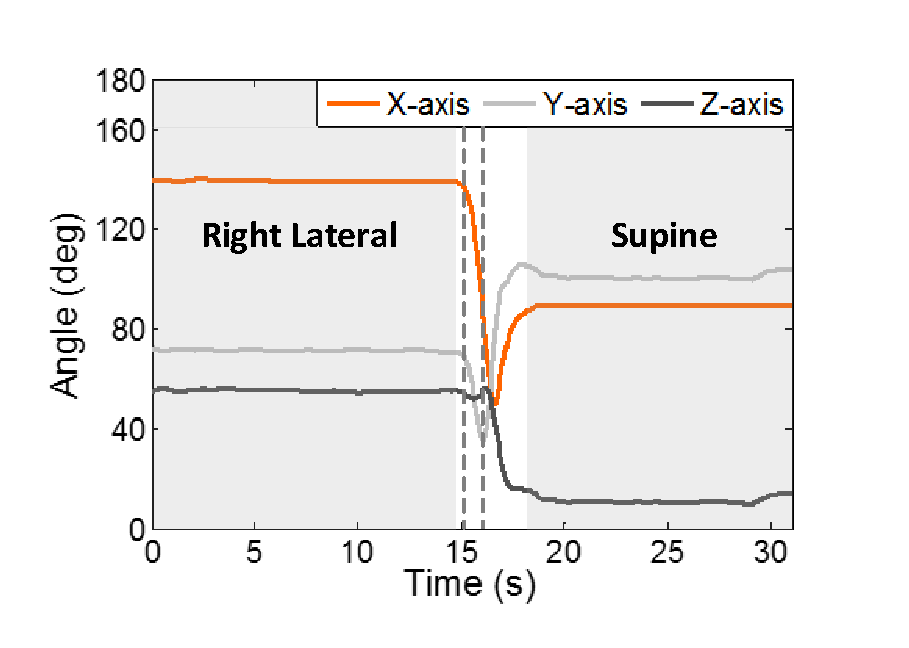
\includegraphics[width=0.97\linewidth]{Figures/RightToSupine.pdf}\centering
  \caption{From right lateral posture to supine posture.}\label{fig:RightToLeft}
\end{minipage}
\end{figure*}

To deal with this challenge, we incorporate the body postures to improve the detection accuracy. As shown in Fig. \ref{fig:BodyRollover},
the body postures are different before and after the rollover. Therefore, after we detect the time when the angle values changes, we term
the time as a possible rollover time point. Then we use the sleep posture classification algorithm to determine whether the body postures
are the same or not over a period of time before and after this point. \textcolor{cyan}{If the postures are the same, we exclude this time
point, otherwise a body rollover event is found. In other words, a body rollover event is recorded when the posture changes are detected
between two time points.} Note that {\systemname} not only counts the number of rollovers, but also reports the exact nature of the
rollover event.


\subsubsection{Detecting micro-body movements \label{sec:microbo}}

Besides major body movement, such as rollovers, there often are involuntary body movements that can affect sleep quality. With the deepening of sleep, limbs are extremely relaxed, and a little stimulus will produce trembling and micro beating. Such behavior is most likely to occur during the deep sleep stage and the REM stage~\cite{ancoli2003role,Jean2000Sleep}. Therefore, by detecting such micro body movements and distinguish them from large body movements can help us to further analyze the user's sleep stage. In this paper, we are interested in the sleep-related body movements including hand moving, arm raising, and body trembling.

\textcolor{cyan}{One of the challenges in detecting the micro-body movements is to cancel the inherent noises brought by the accelerometer.
To cancel the noises, we apply a moving window to the collected accelerometer data points to minimize the impact of the outliers. To
determine the size of the moving window, we apply different parameter settings to our training data. We found that a moving widow with a
size of 35 gives the best average results on our training set. Therefore, we choose to apply a moving window of 35 sample points to the
collected user data and then calculate Root Sum Square (RSS) for the data points within a window:}

\begin{equation}
      Rss(t) =\sqrt{(acc_x(t))^{2}+(acc_y(t))^{2}+(acc_z(t))^{2}},
\end{equation}
$acc_x(t)$, $acc_y(t)$ and $acc_z(t)$ represent the accelerometer sample value of x-axis, y-axis and z-axis at time stamp t respectively.


\textcolor{cyan}{We can obtain the first-order derivative of from the RSS values:}
\begin{equation}
      V(t)=Rss(t)-Rss(t-1).
\end{equation}

Eventually, we set the threshold to be 0.03, which can achieve a satisfactory detection performance. We also observe that the micro movement duration is very short, which lasts less than 2 s.
However, in our body rollover experiments, we find that the average movement duration is 3 s, as shown in Fig. \ref{fig:LeftToRight} - Fig. \ref{fig:RightToLeft}.
Therefore, we can first divide the body movement events into large movement and micro movement by detecting the signal duration time.

\textcolor{cyan}{To distinguish among the micro-body movements of hand movement, arm raising and body trembling, we first consider the
duration of the movement. We observe from our training data that an arm rising action typically takes around 1.8 second, while a hand
movement and a body trembling take around 1 second. Using the duration of the movement, we can distinguish arm rising from the other two
movements. We also find that the body trembling tends to lead to a more drastic change in the accelerometer readings compared to the hand
movement. This observation is depicted in Fig.{fig:micro-move} using samples from one of our training users. Based on this observation, we
then use the change of accelerometer reading to distinguish between the body trembling and the hand movement. We do so by calculating the
first-order derivative of accelerometer data to find out the peak of the acceleration data.  If the peak is great than 1.5 and the duration
of the movement took between 0.8 and 1.2 second, a body trembling is detected; if the peak is less than 1 and the duration of the movement
took between 0.8 and 1.2 second, a hand movement is detected; otherwise, if the duration of the movement took between 1.5 and 2 second, an
arm rising is detected. These thresholds are empirically determined from our training data.}

%\textcolor{blue}{In order to distinguish micro-body movements, including hand movement, arm raising and body trembling, it is very
%intuitive to detect based on the duration of the movement, because we find that the durations of these movements are significantly
%different.
%So we try to use the duration of these movements to perform detection. However, we find that the average duration of the arm rising is 1.8 s, but the duration of the other two types of movement is around 1 s,
% so it is difficult to set a suitable threshold to accurately detect them. Therefore, only through the duration of the movement we can only detect the arm rising with obvious feature.
% For the hand movement, and body trembling is not effective. However, we have found that body  trembling is a sudden movement event, which leads to a more pronounced change in acceleration,
% so we can use acceleration changes to distinguish them based on such an observed fact. Specifically,  as we can see from the figure,  acceleration of body trembling has a more pronounced peak when compared to the hand movement.
% So we perform peak detection on the first-order derivative of the acceleration.}
%
% So we perform peak detection on the acceleration variance. For the detected peak, we calculate the difference $d$ between the peak of the accelerometer data and the average peaks of the accelerometer readings in our training data.
%
%\begin{equation}
%      d=\mid(peak-average(oi))\mid,
%\end{equation}
%$oi$ indicates the type of micro-movement, when $oi$ is 1, it indicates the hand movement and 2 represent body trembling.
%

\begin{figure}[!t]
\centering
      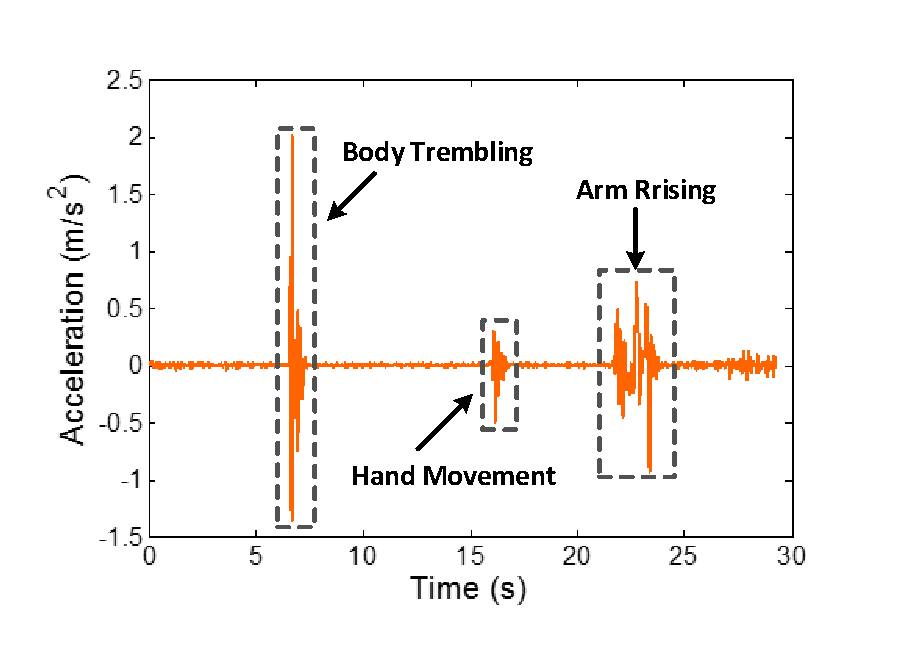
\includegraphics[width=0.43\linewidth]{Figures/Micromovement.pdf}
  \caption{Accelerometer readings for micro body movements using samples from one of our training users.}\label{fig:micro-move}
\end{figure}

%For the two types of potential micro-movements to be classified, we calculate variances for 100 sets of micro-movement data for these 10 volunteers and perform peak detection, as well as make these peaks as features for a particular type of movement to establish a reference data set. In order to classify the micro-movement more accurately, we further obtain the average of the peak features ($average(oi)$) in the reference data set. And then we determine the type of micro-movement with the smallest value of d as the final detection result.


\subsection{Detecting Acoustic Events \label{sec:acoustic}}
Acoustic events during sleep, such as snore, cough and somniloquy, can reflect and affect user's sleep quality and physical health. For
example, snore is one of the possible symptoms of cerebral infarction patients.  And long-term snoring can also have a serious impact on
health and sleep. It can cause behind sleep apnea or narcolepsy, a sleeping disorder~\cite{snoring2016,snoring2013}. And when there is a
cough, the human cerebral cortex cells are always in an excited state, limiting the depth of sleep, allowing only short sleep between
wakefulness, like many other sleep disruptions. {\systemname} can detect these different acoustic events, including snore, cough and
somniloquy. \textcolor{cyan}{ Classical acoustic algorithms use multi-dimensional features to detect acoustic events from a complex
environment~\cite{gu2016sleep}. By contrast, We tailor our design to the problem domain to derive a simpler yet effective acoustic
detection algorithm, by exploiting the characteristics of the different events that we target.}

\begin{figure*}[!t]
\centering
%   \setlength{\abovecaptionskip}{-2pt}
% \setlength{\belowcaptionskip}{-9pt}
%\begin{minipage}[t]{0.32\linewidth}\centering
 \subfigure[Snore of six times.]{\label{snore}
   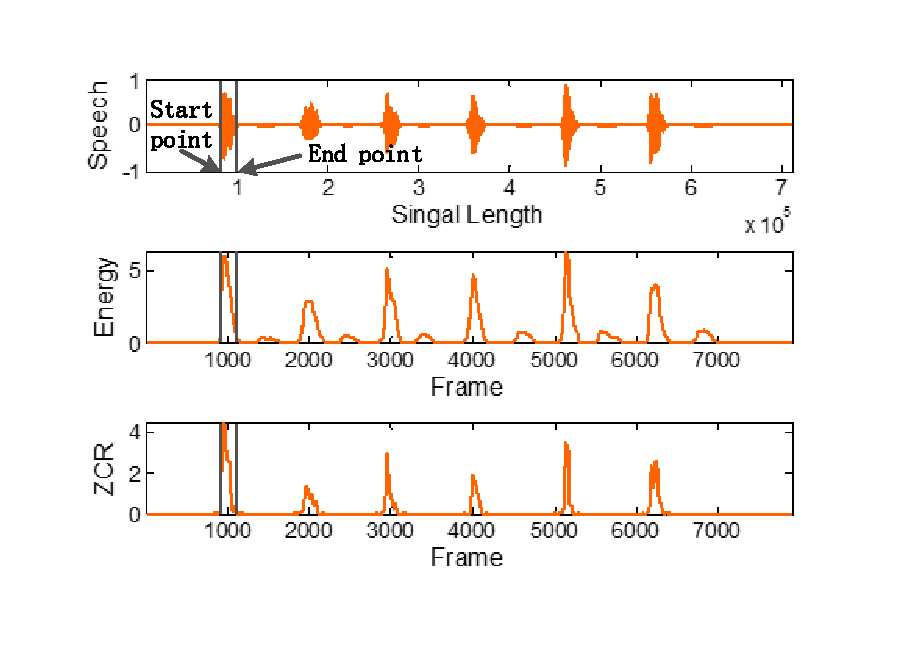
\includegraphics[width=0.32\linewidth]{Figures/snore.pdf}}
 \subfigure[Two consecutive cough.]{\label{cough}
   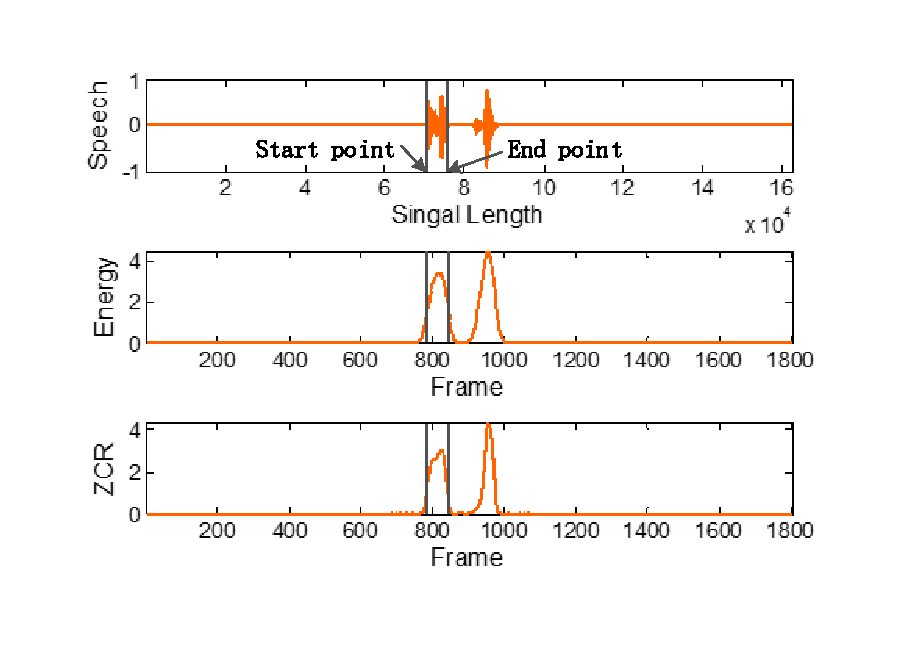
\includegraphics[width=0.32\linewidth]{Figures/cough.pdf}}
\subfigure[Somniloquy.]{\label{somniloquy}
     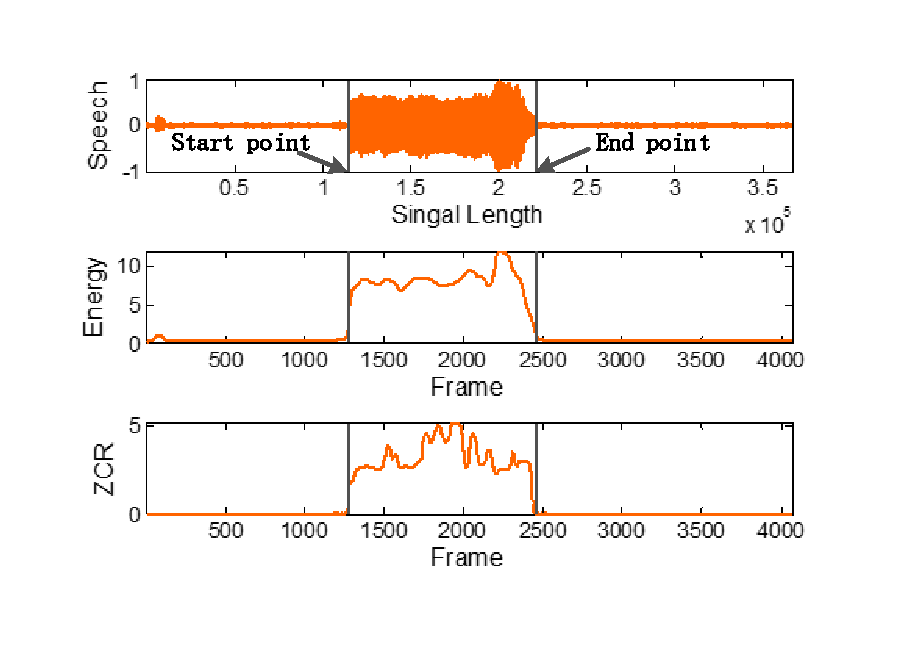
\includegraphics[width=0.32\linewidth]{Figures/somniloquy.pdf}}
\caption{The characteristics of different acoustic events.}\label{acoustic}
\end{figure*}


\subsubsection*{Acoustic feature calculation}
In order to identify different acoustic events accurately, we select the short-term average energy and the zero-crossing rate as two features. The short-term average energy of acoustic signal is computed as:
\begin{equation}
  E_i=\sum\nolimits_{j=-\infty}^{\infty}[x(j)\omega(i-j)]^2=\sum\nolimits_{j=i-(N-1)}^{i}[x(j)\omega(i-j)]^2,
\end{equation}
$N$ is the window length, $x$ is the signal and $\omega$ is the impulse response. As we can see that the short-term energy is the weighted
sum of squared frame sample. The short-term energy can be used to distinguish the segment of unvoiced and voiced sound. It also can be used
to differentiate speech segment and noise segment  in  case of relatively high signal to noise ratio (SNR). The zero-crossing rate is
computed as:
\begin{equation}
  Z_i = \frac{1}{2}\sum\nolimits_{j=0}^{N}|sgn[x_i(j)]-sgn[x_i(j-1)]|.
\end{equation}
It indicates the number of times, which the acoustic signal waveform passes through the horizontal axis (zero level). We carry out an interesting recognition experiment using the microphone built in smartwatch to detect the sound of people during sleep and effectively identify different acoustic events. We focus on three common acoustic events: snore, cough and somniloquy. Ten volunteers worn the smartwatches during sleep to record the acoustic data. We manually label the data with different acoustic events. Fig. \ref{acoustic} shows the acoustic characteristics of  three events. There are six times snore event, two consecutive cough event and somniloquy event.
%The sample rate is 22050 Hz.


\subsubsection*{Acoustic event recognition}
 At beginning, the algorithm  divides the audio stream into frames with equal durations. Each frame is composed of 256 samples, and its duration is 12 ms. To identify the  three common acoustic events, we introduce an acoustic recognition algorithm based on the following key observations:

 \begin{itemize}[itemsep=1mm,nolistsep]
\item The time interval between two signals for different acoustic events are quite different from each other. As shown in Fig.~\ref{snore}, there is a long time interval between two snores. While, the time interval between two coughs is very short.  In contrast, the  somniloquy signal is irregular and without periodic property.
    %Besides, the snore event produces periodic signals and their intervals  are similar.
 \item The duration of one signal for different acoustic events are different from each other. Fig. \ref{acoustic} shows that the duration of a snore is shorter than the duration of a cough and somniloquy. And in general, the duration of a cough is shorter than the duration of a somniloquy signal.
\item The frequencies for different acoustic events are quite different from each other. Snore event has a continuous signal, while the  cough and somniloquy are sudden events, thus the number of consecutive occurrences is very small.
\end{itemize}
In conclusion, the ``interval'', ``duration'' and ``frequency'' of acoustic events can be used as three unique features. Based on the above three observations, our acoustic event recognition algorithm involves the following two steps. First, in order to estimate the interval and frequency of an acoustic event, we perform the peak detection. We use the short-term average energy to calculate the peak value of the acoustic signal. When the peak exceeds a certain threshold, such as 3 dB in this paper, we record the position of each peak and calculate the interval between two consecutive peaks. Next, we can estimate the frequency of an acoustic event by counting the number of peaks over a time window. Second, to estimate the duration of the acoustic event, we perform the start-point and end-point detection.

Traditional end-point detection algorithm \cite{stowell2015detection}, however, uses a fixed double threshold and must be obtained by a
large number of data samples, which has two drawbacks. First, the fixed double threshold may cause error detection at the beginning of
acoustic event. Second, the requirement of a large number of data samples would lead to large system latency. \textcolor{cyan}{To address
these issues, we develop a detection method that does not require pre-sampling to obtain the optimal thresholds. Instead, our algorithm
estimates the thresholds on a per signal basis. This strategy not only reduces the number of data samples needed, but also leads to a
higher accuracy. }

Specifically, since the first few frames and the last few frames are mostly mute or are the background noise, we select the first five
frames and the last five frames to calculate their short-term energy, which are denoted as $E_s$ and $E_e$, respectively. And then the two
are combined to obtain the mean $E_n$ as the estimated energy value of the noise segment.Let the maximum value of the short-term energy
over all frames denoted as $\max (E)$. Then, the average short-term energy $DE$ is given as:
\begin{eqnarray}
      &E_n = \frac{(E_s+E_e)}{2}, \\
      &DE = \max (E)-E_n.\label{eq:DE}
\end{eqnarray}

So we can use $EH$ and $EL$ to represent the high and low threshold of short-term energy, which are given as:
\begin{equation}
      EH=\alpha \times DE+E_n,
\end{equation}
\begin{equation}
    EL=\beta \times DE+E_n,
\end{equation}

 \textcolor{blue}{$\alpha$ and $\beta$ are the multiplier factor of the energy value DE. In order to set the energy threshold for detecting the start and end points of the speech signal, we first need to consider that this threshold must be greater than the energy of the noise signal ($E_n$) to ensure that the noise is filtered out. And then we need to get select the appropriate $\alpha$ and $\beta$ to ensure that we get the proper double threshold to accurately detect the start and end points. Specifically, we used the nighttime sound data of 10 volunteers who participated in training to train the multiplier factor of the energy value DE of the speech signal throughout the frame. We vary $\alpha$ from 0.1 to 0.5 and $\beta$ from 0.01 to 0.09, eventually set $\alpha$ to be 0.1 and $\beta$ to be 0.06, which achieves the best detection performance.}

 Moreover, in order to avoid the interference of sudden noise, we set the minimum length of the signal segment and count the length of the signal during the search for the start and end point. Finally, if the signal length is less than the set minimum, it is considered as a noise segment. The results of the start-point and end-point detection are shown in Fig. \ref{acoustic}, we calculate the length of each speech segment and calculate their averages as the duration of the acoustic event. Last, we count the number of peak points to determine whether it meets the third key observation or not.



%Algorithm 1 provides the detailed  process of the start-point  and end-point detections.


%$A_x$, $A_y$ and $A_z$ are the tilt angle of the three axes, and $\omega_x$, $\omega_y$ and $\omega_z$ are the rotation speed of the three axes. So $\phi$, $\theta$ and $\psi$ are the rotation angle of the three axes. \textcolor[rgb]{1.00,0.00,0.00}{(Those symbols do not present in Algorithm 1)}


%\begin{table}[!thbp]
%\begin{tabular}{l}
%  \hline
%  \textbf{Algorithm 1} The Endpoint Detection \\
%  \hline
%  \textbf{Input}: A sound signal recorded by the microphone:$x$
%  \\\quad \quad \quad The threshold of zero-crossing rate:$ZT$
%  \\\quad \quad \quad The minimum length of speech:$minlen$\\
%  \textbf{Output}:The start-point  and end-point :$p_s,p_e$\\
%  1: Split  $x$ using the framing algorithm \\
%  2: Calculate each frame of energy and zero-crossing rate:$E_i,Z_i$ \\
%  3: Calculate the threshold for short-time energy:$EH,EL$  \\
%  4:$count=0$,$silence=0$\\
%  \textbf{the start point}\\
%  5:\textbf{for}i=1$\rightarrow \frac{length(x)}{frame~length}$  do\\
%  6: \textbf{if} $ E_i>EH $ \textbf{then}\\
%  7: $count=count+1$,$silence = 0$,$max(n-count-1,1)=p_s$\\
%  8: \textbf{else if} $E_i>El || z_i>ZT $\textbf{then}\\
%  9: $count=count+1$ \\
%  10: \textbf{else}\\
%  11:$count=0 $ \\
%  12: \textbf{end if}\\
%  \textbf{the end point}\\
%  13:\textbf{if} $E_i>El || z_i>ZT $\textbf{then}\\
%  14:$count=count+1$ \\
%  15:\textbf{else}\\
%  16:$silence = silence+1 $ \\
%  17:\textbf{if} $count < minlen$\textbf{then}\\
%  18:$count=0 $, $silence=0$ \\
%  19:\textbf{end if}\\
%  20:$count1 = count-\frac{silence}{2}$\\
%  21:$ p_e = p_s + count1 -1$ \\
%  \hline
%\end{tabular}
%\end{table}


\subsection{Tracking Illumination Conditions \label{sec:illumination}}
Studies have shown that there is a significant interaction between illuminance level and the mental state of the individual \cite{light77}.
For example, the bright light can counteract subjective fatigue during daytime, but at night it will seriously affecting the sleep quality.
Too much light exposure can shift our biological clock, which makes restful sleep difficult to achieve, it affects our sleep and wake cycle
\cite{light2007}.  Besides, we also note that the dim light will affect our sleep too. According to the study \cite{light2016}, it can be
learned that the dim artificial light during sleep is significantly associated with the general increase in fatigue, and the proper light
can be used to increase the sense of exhaustion and promote sleep. So illumination condition in a sleeping environment has a significant
influence on sleep. {\systemname} use the ambient light sensor to detect the illumination condition during sleep. We visit 10 volunteers'
bedroom at night and the use of the ambient light sensor to test the lighting conditions in the bedroom, \textcolor{blue}{and we find that
in the absence of light in the bedroom, the reading of the light sensor is basically maintained at 1Lux to 4Lux. In some cases, the watch's
screen is awakened and lighted up to cause the light to rise to 4Lux; when the bedroom is in a faint light, such as a table lamp light, the
light sensor's average readings are also maintained below 10Lux. So ultimately we will divide the illumination intensity into two
conditions: bedroom without light (Weak illumination condition, $\leq$ 10Lux);  bedroom with strong lights (Strong illumination condition,
$>$ 10Lux).} Therefore, we can learn the light conditions in the sleeping environment according to the two types of illumination
conditions.

However, the light sensor may be obscured, which leads to large errors in measuring the illumination level. For example, a user's smartwatch may be covered under quilt when he/she turned over unconsciously, and thus the illumination readings on the smartwatch may not reflect the real lighting situation. \textcolor{blue}{Previous work has used the smartphone to detect the illumination conditions and also encountered the situation where the light sensor was blocked. To deal with this problem, they chose to introduce another sensor in the smartphone, the proximity sensor,  to detect whether the light sensor is blocked or not. However, it does not apply in smartwatch because there is no proximity sensor.} To deal with this practical challenge, the key is that the illumination would drop suddenly when the smartwatch is covered by other objects. There are two possibilities for the sudden drop in light intensity. For most smartwatches, the light sensors are usually installed in the front face of it. The first case is the indoor lighting facilities are closed. The second case is the wrist turned so that the back of the hand become downward, thus blocking the light sensor in front of the smartwatch. \textcolor{blue}{In fact, this situation can easily occur. For example, when a user change sleeping posture to the left side, the user's hand may be close to the pillow with the palm facing up. Or there is a micro body movement like the hand movement so that the back of the hand become downward.} To avoid this erroneous illumination condition measurement, we detect whether the user is performing a wrist flip over a period of time during the intensity plummeting. We detect the wrist flip based on two aspects: (i) the rotation angle of smartwatch; (ii) whether the light intensity maintains stable after the sharp drop. If the wrist flips, we use the average of the previous light intensity as the intensity of the time period. It should be noted that, because the illumination condition detection algorithm is relatively simple, it is not explained in the experimental part.

\subsection{Sleep stage and quality}
\textcolor{blue}{Physiological communities often regard sleep as a cyclical process composed of three stages: rapid eye movement (REM) stage, light sleep stage and deep sleep stage. REM is an active period of sleep marked by intense brain activities and dream occurrence. Light sleep stage is a period of relaxation, when the heartbeat, breathing rate and muscle activity slow down. Deep sleep stage triggers hormones to promote body growth, as well as the repair and restoration of energy.  The biological characteristics of different sleep stages exhibit distinguishingly. In clinical sleep study, the sleep stages are mainly identified by simultaneously evaluating three fundamental measurement modalities including brain activities, eye movements, and muscle contractions. The EEG measure using electrodes placed around the scalp interpret various sleep/wake states of the brain. And, EMG and EOG using electrodes placed on the skin near the eyes and on the muscles, respectively, measures in deeply differentiating REM stage from all the other stages. But, apart from the implicit physiological activities, sleepers usually exhibit distinguishable physical activities in different sleep stages. For example, there are somniloquy and body trembles caused by frequent dreams generally appear in REM, large body movements such as body rollovers and arm raising happen in light sleep and micro body movements such as body trembling and snoring occur in deep sleep.  In the meanwhile, the breathing amplitude in NREM stage is larger compared with the REM stage. Moreover, sleep cycle usually repeats four to six times over a night. The sleeper usually experiences a transition from light sleep to deep sleep and then enters REM, but sometimes there is also possible a phenomenon of skipping some certain sleep stages occurs during sleep. However, despite this, dependence between two successive sleep stages still exists and different sleep stages have potential conversion probabilities, which also mentioned in Sleep Hunter \cite{gu2016sleep}. }

\textcolor{blue}{Thus, based on these features, we build a Hidden Markov Model \cite{johnson2010hidden}. And we use a series of sleep events as the observed sequence and the sleep stage as the implicit stage sequence. $obs_t={NB(t),NB_M(t),BA(t),NA(t)}$ represents the feature vector at detection phase t. The explanation of each item, which is the input of HMM, is listed as follows. $NB(t)$: the number of occurrences of body rollover during the detection phase t. $NB_M(t)$: the number of occurrences of micro body movement. $BA(t)$: the measurement of  respiratory amplitude. $NA(t)$:the number of occurrences acoustic events. And $states_t$ =$\{$light sleep; deep sleep; REM$\}$ is an output of our model, which represents the sleep stage in the detection phase t. In the training of the HMM model, we used nocturnal sleep data from 10 volunteers who participated in the training parameters of each algorithm and make their sleep-related events as observation sequences and the corresponding sleep stages detected by Fitbit as hidden state sequences, to generate HMM models. Specifically, we first use maximum likelihood estimation method for parameter estimation, the state transition matrix and the confusion matrix, and then use the Viterbi algorithm [38] to acquire a series of implicit state sequences corresponding to observed sequence.} As a result, we can estimate the sleep stage during a time window. Finally, we can get the durations of all sleep stages over the whole sleep process.

Further, to quantize the quality of a sleep, we use the Sleep Quality Report model introduced in \cite{gu2016sleep}. Let $SQ$ be the value of the sleep quality, then $SQ$ is given as follow:
 \begin{equation}
SQ=\frac{(REM \times 0.5+Light \times 0.75+Deep) \times 100}{REM+Light+Deep}
 \end{equation}
where, REM, Deep and Light represents the duration time in a sleep process. The range of $SQ$ is from 50 to 100. A high value of $SQ$ shows a good  sleep quality.
